%--------------------INTRODUCTION--------------------------------------
%This is the format for IISER Bhopal PhD Thesis for Physics or Mathematics.
%A modified version of the one originally prepared by Arghya Chattopadhyay (arghya.chattopadhyay@gmail.com). Huge shout out to Arghya for all the hard work!

%Be prepared to modify a bit the IISERB class file to conform with whoever incharge at the academic office PhD section. 

%The formatting related contents (packages, custom layout, fonts, etc.) are now part of the IISERB.cls class file, which also contains the title page layout. 
%All you have to do is enter your details in the individual details section below. 

%This version: 1.0.1 
%Created by: Sandeep Aashish 
%contact: sandeepaashish@hotmail.com
%Date created: January 23, 2020

%--------------------INSTRUCTIONS---------------------------------
%COMPATIBILITY: pdflatex; bibtex; makeindex (for indexing and nomenclature with nomencl package)

%thesis.tex is the mainfile. Other included files (in folders: chapters, frontmatter, endmatter,commands) have a header: %!TEX root=../thesis.tex .
%Most of the required .sty files are in styles folder. Add them to your local latex installation folder (if you don't know how, google it!). 
%bibliography style file hunsrt.bst is also in the styles folder.

%On the first run, follow these steps:
%pdflatex > makeindex thesis.nlo -s nomencl.ist -o thesis.nls > bibtex > pdflatex (x2)

%You can add these arguments for makeindex in your editor's options menu.
%=====================================================================================

\documentclass{IISERB}

\makenomenclature
%For index generation.
%\makeindex 

%====================Set Graphics path============================

\graphicspath{{figures/}}


%=====================Command Modification=========================

%Either enter your modifications here or write them in a seperate file and include it here.

%!TEX root = ../thesis.tex

% Custom commands file. \include in mainfile

%=====================Command Modification=========================

%Either enter your modifications here or write them in a seperate file and include it here. Examples are written below

\newcommand{\be}{\begin{equation}}
\newcommand{\ee}{\end{equation}}

\newcommand{\e}{\epsilon}
\newcommand{\ve}{\varepsilon}
% Set Theoretic Math
\newcommand{\mR}{\mathbb{R}}
\newcommand{\mC}{\mathbb{C}}
\newcommand{\mQ}{\mathbb{Q}}
\newcommand{\mZ}{\mathbb{Z}}
\newcommand{\mN}{\mathbb{N}}



%===============================================================


%=====================For Dummy text, tables and figures===============
%One can comment this section out

%\usepackage{lipsum}
%\usepackage{sator}

%===============================================================



% ------------------------------
% Individual details (Change these!)
% ------------------------------

% don't forget to remove the square brackets

\newcommand{\thesistitle}{[Thesis Title]}%Include your thesis title
\newcommand{\studentname}{[Student Name]}%Change it to your name
\newcommand{\salutation}{[Mr./Ms.]}% Mr. or Ms. or anything
\newcommand{\studentrollno}{[Roll Number]}%Change it to your roll number
\newcommand{\advisorname}{[Supervisor]}%Change it to your advisor's name
\newcommand{\subject}{[Department]}%Change it to physics or maths
\newcommand{\thesisdate}{[Month, year]}%Include thesis year
\newcommand{\vivadate}{[Month, year]}%Include viva date, keep it same as the thesis date while forwarding for evaluation
\newcommand{\thesisyear}{[year]}%Again input the year for convinience
\newcommand{\external}{[name of Ex. Examiner]}%Input the name of external examiner
\newcommand{\memberone}{[name of the oral board examiner]}%Input the name of the member
\newcommand{\membertwo}{[name of the oral board examiner]}%Input the name of the member
\newcommand{\memberthre}{[name of the oral board examiner]]}%Input the name of the member




\begin{document}



\begin{titlepage}
\maketitle
\end{titlepage}
%%%%%%%%%%%%% 2nd title %%%%%%%%%%%%%
\newpage
\begin{titlepage}
\maketitle
\end{titlepage}



\pagebreak
%!TEX root=../thesis.tex

%\vspace{2cm}
\begin{center}\Large{\textbf{CERTIFICATE}}\end{center}
\vspace{0.5cm}
The undersigned have examined the Ph.D. thesis entitled:
\begin{center}\textbf{\thesistitle}\end{center}
presented by \salutation \studentname, a candidate for the degree of \mbox{Doctor of Philosophy} in the department of \subject, and hereby certify that it is worthy of acceptance.

\vspace{1cm}
\parbox{0.6\textwidth}{ 
\flushleft{\vivadate\\IISER, Bhopal}
\vspace{16cm}
}
\hfill 
\parbox{0.4\textwidth}{ 
\mbox{\external}\\
External Examiner\\

\vspace{1.3cm}
\mbox{\advisorname}\\
Supervisor\\

\vspace{1.3cm}
\mbox{\memberone}\\
Member\\

\vspace{1.3cm}
\mbox{\membertwo}\\
Member\\

\vspace{1.3cm}
\mbox{\memberthre}\\
Member\\
}

\addcontentsline{toc}{chapter}{Certificate}
\newpage  
\addcontentsline{toc}{chapter}{Academic Integrity and Copyright Disclaimer}
%!TEX root=../thesis.tex


%\hspace{2cm}
\begin{center}
{\textbf{\Large{ACADEMIC INTEGRITY AND COPYRIGHT DISCLAIMER}}}
 \end{center}
I hereby declare that this thesis is my own work and, to the best of my knowledge, it contains no materials previously published or written by any other person, or substantial proportions of material which have been accepted for the award of any other degree or diploma at IISER Bhopal or any other educational institution, except where due acknowledgement is made in the thesis. \\ \\
I certify that all copyrighted material incorporated into this thesis is in compliance with the Indian Copyright (Amendment) Act, 2012 and that I have received written permission from the copyright owners for my use of their work, which is beyond the scope of the law. I agree to indemnify and save harmless IISER Bhopal from any and all claims that may be asserted or that may arise from any copyright violation.

\vspace{2cm}
\parbox{0.7\textwidth}{ 
	\flushleft{\thesisdate\\IISER, Bhopal}
}
\hfill 
\parbox{0.3\textwidth}{ 
	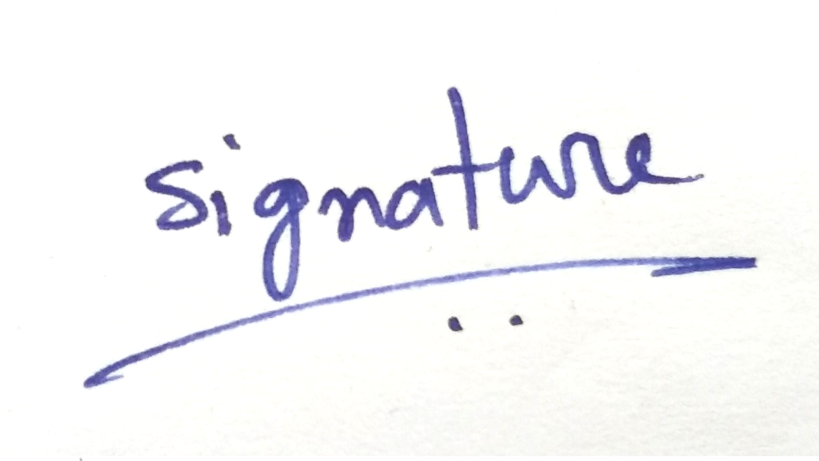
\includegraphics[width=5cm]{sign}
\mbox{\studentname}
}
\newpage
\addcontentsline{toc}{chapter}{Acknowledgement}
%!TEX root=../thesis.tex


\begin{center}
{\textbf{\large{ACKNOWLEDGEMENTS}}}
 \end{center}
 Put the acknowledgement
\newpage
\addcontentsline{toc}{chapter}{Dedication}
%!TEX root=../thesis.tex


\begin{dedication}
    Dedicated to the dedicated
\end{dedication}


\newpage 
\addcontentsline{toc}{chapter}{Abstract}
%!TEX root=../thesis.tex

\begin{center}\Large{\textbf{ABSTRACT}}\end{center}
Abstract
\newpage
\addcontentsline{toc}{chapter}{Table of Contents}
\tableofcontents
\newpage


%====================Symbols================================

\addcontentsline{toc}{chapter}{List of Symbols and Abbreviations}%

%!TEX root = ../thesis.tex
%Add your own nomenclatures

%====================Symbols================================
%Below is the example to add nomenclature entries. You can add them in the main text as well in this same format.

\begin{center}\Large{\textbf{List of Symbols \& Abbreviations}}\end{center}

\nomenclature{$k_B$}{Boltzmann constant} 
\nomenclature{$T$}{Temperature} 
\nomenclature{$\epsilon$}{Energy parameter} 
\nomenclature{$\alpha$}{alpha particle} 

\printnomenclature

%============================================================



%=============Generating List of figures and list of tables================
\addcontentsline{toc}{chapter}{List of Figures}
\listoffigures

\addcontentsline{toc}{chapter}{List of Tables}
\listoftables

\pagestyle{fancy}
\clearpage
\pagenumbering{arabic}


%=====================Chapters==============================================
\newpage


%!TEX root = ../thesis.tex

\chapter{The title of chapter one}


Lorem ipsum dolor sit amet \cite{dummy}, consectetuer adipiscing elit. Morbi commodo, ipsum sed pharetra gravida, orci magna rhoncus neque, id pulvinar odio lorem non turpis. Nullam sit amet enim. Suspendisse id velit vitae ligula volutpat condimentum. Aliquam erat volutpat. Sed quis velit. Nulla facilisi. Nulla libero. Vivamus pharetra posuere sapien. Nam consectetuer. Sed aliquam, nunc eget euismod ullamcorper, lectus nunc ullamcorper orci, fermentum bibendum enim nibh eget ipsum. Donec porttitor ligula eu dolor. Maecenas vitae nulla consequat libero cursus venenatis. Nam magna enim, accumsan eu, blandit sed, blandit a, eros.

Quisque facilisis erat a dui. Nam malesuada ornare dolor. Cras gravida, diam sit amet rhoncus ornare, erat elit consectetuer erat, id egestas pede nibh eget odio. Proin tincidunt, velit vel porta elementum, magna diam molestie sapien, non aliquet massa pede eu diam. Aliquam iaculis. Fusce et ipsum et nulla tristique facilisis. Donec eget sem sit amet ligula viverra gravida. Etiam vehicula urna vel turpis. Suspendisse sagittis ante a urna. Morbi a est quis orci consequat rutrum. Nullam egestas feugiat felis. Integer adipiscing semper ligula. Nunc molestie, nisl sit amet cursus convallis, sapien lectus pretium metus, vitae pretium enim wisi id lectus. Donec vestibulum. Etiam vel nibh. Nulla facilisi. Mauris pharetra. Donec augue. Fusce ultrices, neque id dignissim ultrices, tellus mauris dictum elit, vel lacinia enim metus eu nunc.

Pellentesque habitant morbi tristique senectus et netus et malesuada fames ac turpis egestas. Vestibulum tortor quam, feugiat vitae, ultricies eget, tempor sit amet, ante. Donec eu libero sit amet quam egestas semper. Aenean ultricies mi vitae est. Mauris placerat eleifend leo. Quisque sit amet est et sapien ullamcorper pharetra. Vestibulum erat wisi, condimentum sed, commodo vitae, ornare sit amet, wisi. Aenean fermentum, elit eget tincidunt condimentum, eros ipsum rutrum orci, sagittis tempus lacus enim ac dui. Donec non enim in turpis pulvinar facilisis. Ut felis.

Cras sed ante. Phasellus in massa. Curabitur dolor eros, gravida et, hendrerit ac, cursus non, massa. Aliquam lorem. In hac habitasse platea dictumst. Cras eu mauris. Quisque lacus. Donec ipsum. Nullam vitae sem at nunc pharetra ultricies. Vivamus elit eros, ullamcorper a, adipiscing sit amet, porttitor ut, nibh. Maecenas adipiscing mollis massa. Nunc ut dui eget nulla venenatis aliquet. Sed luctus posuere justo. Cras vehicula varius turpis. Vivamus eros metus, tristique sit amet, molestie dignissim, malesuada et, urna.

Cras dictum. Maecenas ut turpis. In vitae erat ac orci dignissim eleifend. Nunc quis justo. Sed vel ipsum in purus tincidunt pharetra. Sed pulvinar, felis id consectetuer malesuada, enim nisl mattis elit, a facilisis tortor nibh quis leo. Sed augue lacus, pretium vitae, molestie eget, rhoncus quis, elit. Donec in augue. Fusce orci wisi, ornare id, mollis vel, lacinia vel, massa.

Lorem ipsum dolor sit amet, consectetuer adipiscing elit. Morbi commodo, ipsum sed pharetra gravida, orci magna rhoncus neque, id pulvinar odio lorem non turpis. Nullam sit amet enim. Suspendisse id velit vitae ligula volutpat condimentum. Aliquam erat volutpat. Sed quis velit. Nulla facilisi. Nulla libero. Vivamus pharetra posuere sapien. Nam consectetuer. Sed aliquam, nunc eget euismod ullamcorper, lectus nunc ullamcorper orci, fermentum bibendum enim nibh eget ipsum. Donec porttitor ligula eu dolor. Maecenas vitae nulla consequat libero cursus venenatis. Nam magna enim, accumsan eu, blandit sed, blandit a, eros.

Quisque facilisis erat a dui. Nam malesuada ornare dolor. Cras gravida, diam sit amet rhoncus ornare, erat elit consectetuer erat, id egestas pede nibh eget odio. Proin tincidunt, velit vel porta elementum, magna diam molestie sapien, non aliquet massa pede eu diam. Aliquam iaculis. Fusce et ipsum et nulla tristique facilisis. Donec eget sem sit amet ligula viverra gravida. Etiam vehicula urna vel turpis. Suspendisse sagittis ante a urna. Morbi a est quis orci consequat rutrum. Nullam egestas feugiat felis. Integer adipiscing semper ligula. Nunc molestie, nisl sit amet cursus convallis, sapien lectus pretium metus, vitae pretium enim wisi id lectus. Donec vestibulum. Etiam vel nibh. Nulla facilisi. Mauris pharetra. Donec augue. Fusce ultrices, neque id dignissim ultrices, tellus mauris dictum elit, vel lacinia enim metus eu nunc.

\texttt{This is a line of code.}

Proin at eros non eros adipiscing mollis. Donec semper turpis sed diam. Sed consequat ligula nec tortor. Integer eget sem. Ut vitae enim eu est vehicula gravida. Morbi ipsum ipsum, porta nec, tempor id, auctor vitae, purus. Pellentesque neque. Nulla luctus erat vitae libero. Integer nec enim. Phasellus aliquam enim et tortor. Quisque aliquet, quam elementum condimentum feugiat, tellus odio consectetuer wisi, vel nonummy sem neque in elit. Curabitur eleifend wisi iaculis ipsum. Pellentesque habitant morbi tristique senectus et netus et malesuada fames ac turpis egestas. In non velit non ligula laoreet ultrices. Praesent ultricies facilisis nisl. Vivamus luctus elit sit amet mi. Phasellus pellentesque, erat eget elementum volutpat, dolor nisl porta neque, vitae sodales ipsum nibh in ligula. Maecenas mattis pulvinar diam. Curabitur sed leo.

Nulla facilisi. In vel sem. Morbi id urna in diam dignissim feugiat. Proin molestie tortor eu velit. Aliquam erat volutpat. Nullam ultrices, diam tempus vulputate egestas, eros pede varius leo, sed imperdiet lectus est ornare odio. Lorem ipsum dolor sit amet, consectetuer adipiscing elit. Proin consectetuer velit in dui. Phasellus wisi purus, interdum vitae, rutrum accumsan, viverra in, velit. Sed enim risus, congue non, tristique in, commodo eu, metus. Aenean tortor mi, imperdiet id, gravida eu, posuere eu, felis. Mauris sollicitudin, turpis in hendrerit sodales, lectus ipsum pellentesque ligula, sit amet scelerisque urna nibh ut arcu. Aliquam in lacus. Vestibulum ante ipsum primis in faucibus orci luctus et ultrices posuere cubilia Curae; Nulla placerat aliquam wisi. Mauris viverra odio. Quisque fermentum pulvinar odio. Proin posuere est vitae ligula. Etiam euismod. Cras a eros.

Nunc auctor bibendum eros. Maecenas porta accumsan mauris. Etiam enim enim, elementum sed, bibendum quis, rhoncus non, metus. Fusce neque dolor, adipiscing sed, consectetuer et, lacinia sit amet, quam. Suspendisse wisi quam, consectetuer in, blandit sed, suscipit eu, eros. Etiam ligula enim, tempor ut, blandit nec, mollis eu, lectus. Nam cursus. Vivamus iaculis. Aenean risus purus, pharetra in, blandit quis, gravida a, turpis. Donec nisl. Aenean eget mi. Fusce mattis est id diam. Phasellus faucibus interdum sapien. Duis quis nunc. Sed enim.

Pellentesque vel dui sed orci faucibus iaculis. Suspendisse dictum magna id purus tincidunt rutrum. Nulla congue. Vivamus sit amet lorem posuere dui vulputate ornare. Phasellus mattis sollicitudin ligula. Duis dignissim felis et urna. Integer adipiscing congue metus. Nam pede. Etiam non wisi. Sed accumsan dolor ac augue. Pellentesque eget lectus. Aliquam nec dolor nec tellus ornare venenatis. Nullam blandit placerat sem. Curabitur quis ipsum. Mauris nisl tellus, aliquet eu, suscipit eu, ullamcorper quis, magna. Mauris elementum, pede at sodales vestibulum, nulla tortor congue massa, quis pellentesque odio dui id est. Cras faucibus augue.

Suspendisse vestibulum dignissim quam. Integer vel augue. Phasellus nulla purus, interdum ac, venenatis non, varius rutrum, leo. Pellentesque habitant morbi tristique senectus et netus et malesuada fames ac turpis egestas. Duis a eros. Class aptent taciti sociosqu ad litora torquent per conubia nostra, per inceptos hymenaeos. Fusce magna mi, porttitor quis, convallis eget, sodales ac, urna. Phasellus luctus venenatis magna. Vivamus eget lacus. Nunc tincidunt convallis tortor. Duis eros mi, dictum vel, fringilla sit amet, fermentum id, sem. Phasellus nunc enim, faucibus ut, laoreet in, consequat id, metus. Vivamus dignissim. Cras lobortis tempor velit. Phasellus nec diam ac nisl lacinia tristique. Nullam nec metus id mi dictum dignissim. Nullam quis wisi non sem lobortis condimentum. Phasellus pulvinar, nulla non aliquam eleifend, tortor wisi scelerisque felis, in sollicitudin arcu ante lacinia leo.

Pellentesque habitant morbi tristique senectus et netus et malesuada fames ac turpis egestas. Vestibulum tortor quam, feugiat vitae, ultricies eget, tempor sit amet, ante. Donec eu libero sit amet quam egestas semper. Aenean ultricies mi vitae est. Mauris placerat eleifend leo. Quisque sit amet est et sapien ullamcorper pharetra. Vestibulum erat wisi, condimentum sed, commodo vitae, ornare sit amet, wisi. Aenean fermentum, elit eget tincidunt condimentum, eros ipsum rutrum orci, sagittis tempus lacus enim ac dui. Donec non enim in turpis pulvinar facilisis. Ut felis.

Cras sed ante. Phasellus in massa. Curabitur dolor eros, gravida et, hendrerit ac, cursus non, massa. Aliquam lorem. In hac habitasse platea dictumst. Cras eu mauris. Quisque lacus. Donec ipsum. Nullam vitae sem at nunc pharetra ultricies. Vivamus elit eros, ullamcorper a, adipiscing sit amet, porttitor ut, nibh. Maecenas adipiscing mollis massa. Nunc ut dui eget nulla venenatis aliquet. Sed luctus posuere justo. Cras vehicula varius turpis. Vivamus eros metus, tristique sit amet, molestie dignissim, malesuada et, urna.

Cras dictum. Maecenas ut turpis. In vitae erat ac orci dignissim eleifend. Nunc quis justo. Sed vel ipsum in purus tincidunt pharetra. Sed pulvinar, felis id consectetuer malesuada, enim nisl mattis elit, a facilisis tortor nibh quis leo. Sed augue lacus, pretium vitae, molestie eget, rhoncus quis, elit. Donec in augue. Fusce orci wisi, ornare id, mollis vel, lacinia vel, massa.

Lorem ipsum dolor sit amet, consectetuer adipiscing elit. Morbi commodo, ipsum sed pharetra gravida, orci magna rhoncus neque, id pulvinar odio lorem non turpis. Nullam sit amet enim. Suspendisse id velit vitae ligula volutpat condimentum. Aliquam erat volutpat. Sed quis velit. Nulla facilisi. Nulla libero. Vivamus pharetra posuere sapien. Nam consectetuer. Sed aliquam, nunc eget euismod ullamcorper, lectus nunc ullamcorper orci, fermentum bibendum enim nibh eget ipsum. Donec porttitor ligula eu dolor. Maecenas vitae nulla consequat libero cursus venenatis. Nam magna enim, accumsan eu, blandit sed, blandit a, eros.


\begin{figure}
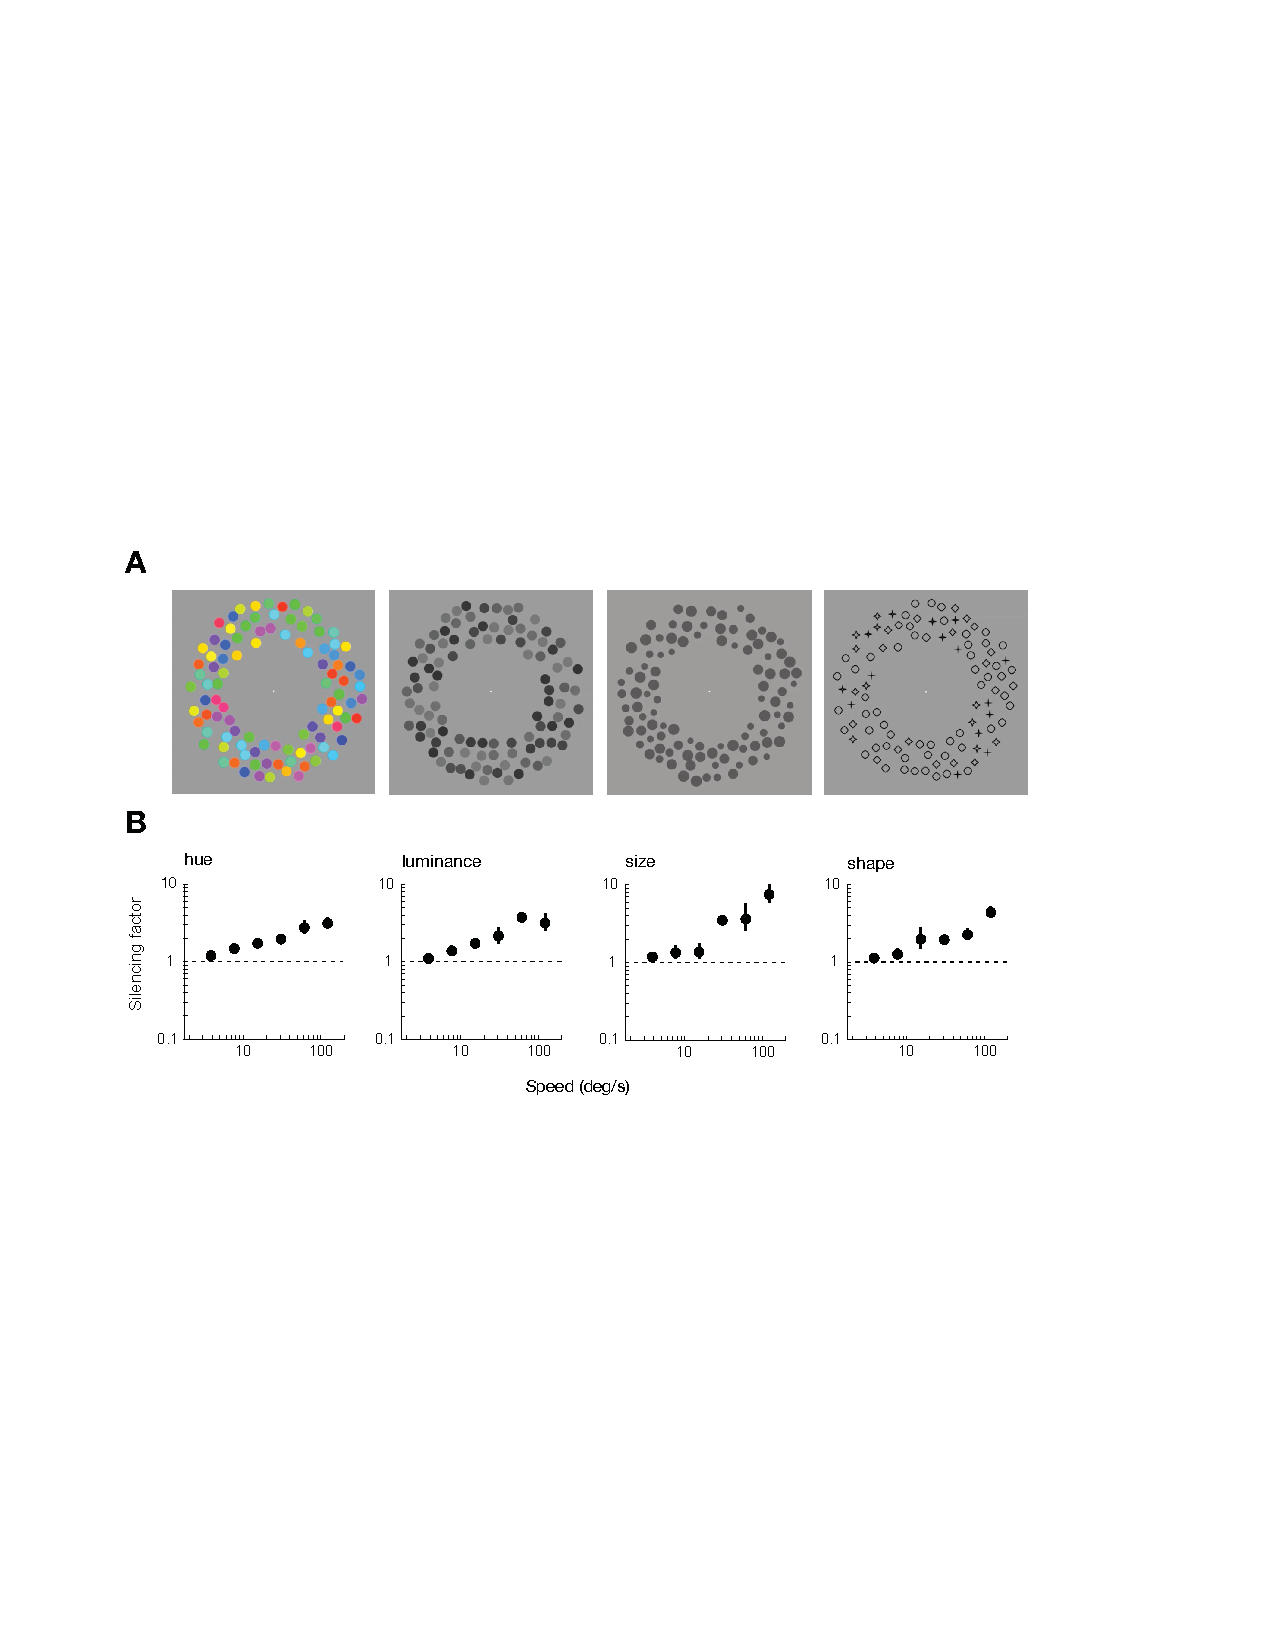
\includegraphics[width=\textwidth]{figures/fig1}
\caption[Short figure name.]{This is a figure that floats inline and here is its caption.
\label{fig:myInlineFigure}}
\end{figure}


Quisque facilisis erat a dui. Nam malesuada ornare dolor. Cras gravida, diam sit amet rhoncus ornare, erat elit consectetuer erat, id egestas pede nibh eget odio. Proin tincidunt, velit vel porta elementum, magna diam molestie sapien, non aliquet massa pede eu diam. Aliquam iaculis. Fusce et ipsum et nulla tristique facilisis. Donec eget sem sit amet ligula viverra gravida. Etiam vehicula urna vel turpis. Suspendisse sagittis ante a urna. Morbi a est quis orci consequat rutrum. Nullam egestas feugiat felis. Integer adipiscing semper ligula. Nunc molestie, nisl sit amet cursus convallis, sapien lectus pretium metus, vitae pretium enim wisi id lectus. Donec vestibulum. Etiam vel nibh. Nulla facilisi. Mauris pharetra. Donec augue. Fusce ultrices, neque id dignissim ultrices, tellus mauris dictum elit, vel lacinia enim metus eu nunc.

Proin at eros non eros adipiscing mollis. Donec semper turpis sed diam. Sed consequat ligula nec tortor. Integer eget sem. Ut vitae enim eu est vehicula gravida. Morbi ipsum ipsum, porta nec, tempor id, auctor vitae, purus. Pellentesque neque. Nulla luctus erat vitae libero. Integer nec enim. Phasellus aliquam enim et tortor. Quisque aliquet, quam elementum condimentum feugiat, tellus odio consectetuer wisi, vel nonummy sem neque in elit. Curabitur eleifend wisi iaculis ipsum. Pellentesque habitant morbi tristique senectus et netus et malesuada fames ac turpis egestas. In non velit non ligula laoreet ultrices. Praesent ultricies facilisis nisl. Vivamus luctus elit sit amet mi. Phasellus pellentesque, erat eget elementum volutpat, dolor nisl porta neque, vitae sodales ipsum nibh in ligula. Maecenas mattis pulvinar diam. Curabitur sed leo.

Nulla facilisi. In vel sem. Morbi id urna in diam dignissim feugiat. Proin molestie tortor eu velit. Aliquam erat volutpat. Nullam ultrices, diam tempus vulputate egestas, eros pede varius leo, sed imperdiet lectus est ornare odio. Lorem ipsum dolor sit amet, consectetuer adipiscing elit. Proin consectetuer velit in dui. Phasellus wisi purus, interdum vitae, rutrum accumsan, viverra in, velit. Sed enim risus, congue non, tristique in, commodo eu, metus. Aenean tortor mi, imperdiet id, gravida eu, posuere eu, felis. Mauris sollicitudin, turpis in hendrerit sodales, lectus ipsum pellentesque ligula, sit amet scelerisque urna nibh ut arcu. Aliquam in lacus. Vestibulum ante ipsum primis in faucibus orci luctus et ultrices posuere cubilia Curae; Nulla placerat aliquam wisi. Mauris viverra odio. Quisque fermentum pulvinar odio. Proin posuere est vitae ligula. Etiam euismod. Cras a eros.

Nunc auctor bibendum eros. Maecenas porta accumsan mauris. Etiam enim enim, elementum sed, bibendum quis, rhoncus non, metus. Fusce neque dolor, adipiscing sed, consectetuer et, lacinia sit amet, quam. Suspendisse wisi quam, consectetuer in, blandit sed, suscipit eu, eros. Etiam ligula enim, tempor ut, blandit nec, mollis eu, lectus. Nam cursus. Vivamus iaculis. Aenean risus purus, pharetra in, blandit quis, gravida a, turpis. Donec nisl. Aenean eget mi. Fusce mattis est id diam. Phasellus faucibus interdum sapien. Duis quis nunc. Sed enim.

Pellentesque vel dui sed orci faucibus iaculis. Suspendisse dictum magna id purus tincidunt rutrum. Nulla congue. Vivamus sit amet lorem posuere dui vulputate ornare. Phasellus mattis sollicitudin ligula. Duis dignissim felis et urna. Integer adipiscing congue metus. Nam pede. Etiam non wisi. Sed accumsan dolor ac augue. Pellentesque eget lectus. Aliquam nec dolor nec tellus ornare venenatis. Nullam blandit placerat sem. Curabitur quis ipsum. Mauris nisl tellus, aliquet eu, suscipit eu, ullamcorper quis, magna. Mauris elementum, pede at sodales vestibulum, nulla tortor congue massa, quis pellentesque odio dui id est. Cras faucibus augue.

%% Requires fltpage2 package
%%
% \begin{FPfigure}
% 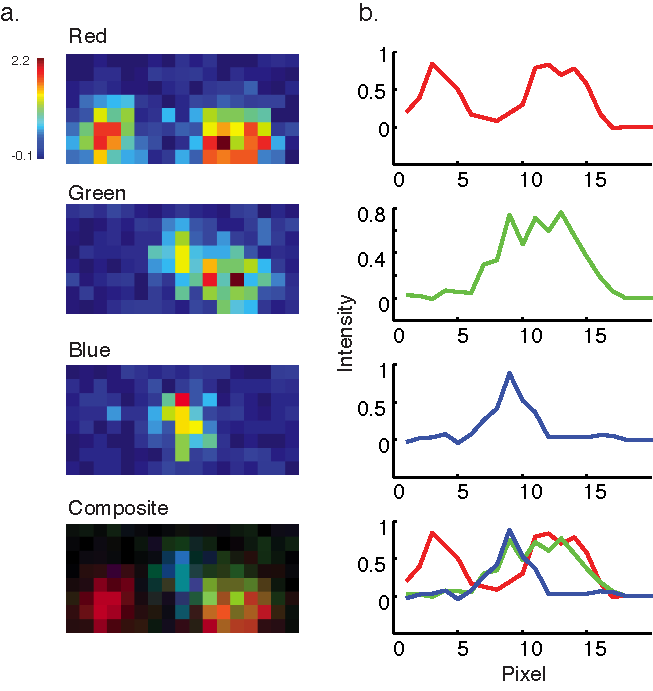
\includegraphics[width=\textwidth]{figures/fullpage}
% \caption[Short figure name.]{This is a full page figure using the FPfigure command. It takes up the whole page and the caption appears on the preceding page. Its useful for large figures. Harvard's rules about full page figures are tricky, but you don't have to worry about it because we took care of it for you. For example, the full figure is supposed to have a title in the same style as the caption but without the actual caption. The caption is supposed to appear alone on the preceding page with no other text. You do't have to worry about any of that. We have modified the fltpage package to make it work. This is a lengthy caption and it clearly would not fit on the same page as the figure. Note that you should only use the FPfigure command in instances where the figure really is too large. If the figure is small enough to fit by the caption than it does not produce the desired effect. Good luck with your thesis. I have to keep writing this to make the caption really long. LaTex is a lot of fun. You will enjoy working with it. Good luck on your post doctoral life! I am looking forward to mine. \label{fig:myFullPageFigure}}
% \end{FPfigure}
% \afterpage{\clearpage}

Suspendisse vestibulum dignissim quam. Integer vel augue. Phasellus nulla purus, interdum ac, venenatis non, varius rutrum, leo. Pellentesque habitant morbi tristique senectus et netus et malesuada fames ac turpis egestas. Duis a eros. Class aptent taciti sociosqu ad litora torquent per conubia nostra, per inceptos hymenaeos. Fusce magna mi, porttitor quis, convallis eget, sodales ac, urna. Phasellus luctus venenatis magna. Vivamus eget lacus. Nunc tincidunt convallis tortor. Duis eros mi, dictum vel, fringilla sit amet, fermentum id, sem. Phasellus nunc enim, faucibus ut, laoreet in, consequat id, metus. Vivamus dignissim. Cras lobortis tempor velit. Phasellus nec diam ac nisl lacinia tristique. Nullam nec metus id mi dictum dignissim. Nullam quis wisi non sem lobortis condimentum. Phasellus pulvinar, nulla non aliquam eleifend, tortor wisi scelerisque felis, in sollicitudin arcu ante lacinia leo.

Pellentesque habitant morbi tristique senectus et netus et malesuada fames ac turpis egestas. Vestibulum tortor quam, feugiat vitae, ultricies eget, tempor sit amet, ante. Donec eu libero sit amet quam egestas semper. Aenean ultricies mi vitae est. Mauris placerat eleifend leo. Quisque sit amet est et sapien ullamcorper pharetra. Vestibulum erat wisi, condimentum sed, commodo vitae, ornare sit amet, wisi. Aenean fermentum, elit eget tincidunt condimentum, eros ipsum rutrum orci, sagittis tempus lacus enim ac dui. Donec non enim in turpis pulvinar facilisis. Ut felis.

Cras sed ante. Phasellus in massa. Curabitur dolor eros, gravida et, hendrerit ac, cursus non, massa. Aliquam lorem. In hac habitasse platea dictumst. Cras eu mauris. Quisque lacus. Donec ipsum. Nullam vitae sem at nunc pharetra ultricies. Vivamus elit eros, ullamcorper a, adipiscing sit amet, porttitor ut, nibh. Maecenas adipiscing mollis massa. Nunc ut dui eget nulla venenatis aliquet. Sed luctus posuere justo. Cras vehicula varius turpis. Vivamus eros metus, tristique sit amet, molestie dignissim, malesuada et, urna.

Proin at eros non eros adipiscing mollis. Donec semper turpis sed diam. Sed consequat ligula nec tortor. Integer eget sem. Ut vitae enim eu est vehicula gravida. Morbi ipsum ipsum, porta nec, tempor id, auctor vitae, purus. Pellentesque neque. Nulla luctus erat vitae libero. Integer nec enim. Phasellus aliquam enim et tortor. Quisque aliquet, quam elementum condimentum feugiat, tellus odio consectetuer wisi, vel nonummy sem neque in elit. Curabitur eleifend wisi iaculis ipsum. Pellentesque habitant morbi tristique senectus et netus et malesuada fames ac turpis egestas. In non velit non ligula laoreet ultrices. Praesent ultricies facilisis nisl. Vivamus luctus elit sit amet mi. Phasellus pellentesque, erat eget elementum volutpat, dolor nisl porta neque, vitae sodales ipsum nibh in ligula. Maecenas mattis pulvinar diam. Curabitur sed leo.

Nulla facilisi. In vel sem. Morbi id urna in diam dignissim feugiat. Proin molestie tortor eu velit. Aliquam erat volutpat. Nullam ultrices, diam tempus vulputate egestas, eros pede varius leo, sed imperdiet lectus est ornare odio. Lorem ipsum dolor sit amet, consectetuer adipiscing elit. Proin consectetuer velit in dui. Phasellus wisi purus, interdum vitae, rutrum accumsan, viverra in, velit. Sed enim risus, congue non, tristique in, commodo eu, metus. Aenean tortor mi, imperdiet id, gravida eu, posuere eu, felis. Mauris sollicitudin, turpis in hendrerit sodales, lectus ipsum pellentesque ligula, sit amet scelerisque urna nibh ut arcu. Aliquam in lacus. Vestibulum ante ipsum primis in faucibus orci luctus et ultrices posuere cubilia Curae; Nulla placerat aliquam wisi. Mauris viverra odio. Quisque fermentum pulvinar odio. Proin posuere est vitae ligula. Etiam euismod. Cras a eros.

Nunc auctor bibendum eros. Maecenas porta accumsan mauris. Etiam enim enim, elementum sed, bibendum quis, rhoncus non, metus. Fusce neque dolor, adipiscing sed, consectetuer et, lacinia sit amet, quam. Suspendisse wisi quam, consectetuer in, blandit sed, suscipit eu, eros. Etiam ligula enim, tempor ut, blandit nec, mollis eu, lectus. Nam cursus. Vivamus iaculis. Aenean risus purus, pharetra in, blandit quis, gravida a, turpis. Donec nisl. Aenean eget mi. Fusce mattis est id diam. Phasellus faucibus interdum sapien. Duis quis nunc. Sed enim.

Pellentesque vel dui sed orci faucibus iaculis. Suspendisse dictum magna id purus tincidunt rutrum. Nulla congue. Vivamus sit amet lorem posuere dui vulputate ornare. Phasellus mattis sollicitudin ligula. Duis dignissim felis et urna. Integer adipiscing congue metus. Nam pede. Etiam non wisi. Sed accumsan dolor ac augue. Pellentesque eget lectus. Aliquam nec dolor nec tellus ornare venenatis. Nullam blandit placerat sem. Curabitur quis ipsum. Mauris nisl tellus, aliquet eu, suscipit eu, ullamcorper quis, magna. Mauris elementum, pede at sodales vestibulum, nulla tortor congue massa, quis pellentesque odio dui id est. Cras faucibus augue.

Suspendisse vestibulum dignissim quam. Integer vel augue. Phasellus nulla purus, interdum ac, venenatis non, varius rutrum, leo. Pellentesque habitant morbi tristique senectus et netus et malesuada fames ac turpis egestas. Duis a eros. Class aptent taciti sociosqu ad litora torquent per conubia nostra, per inceptos hymenaeos. Fusce magna mi, porttitor quis, convallis eget, sodales ac, urna. Phasellus luctus venenatis magna. Vivamus eget lacus. Nunc tincidunt convallis tortor. Duis eros mi, dictum vel, fringilla sit amet, fermentum id, sem. Phasellus nunc enim, faucibus ut, laoreet in, consequat id, metus. Vivamus dignissim. Cras lobortis tempor velit. Phasellus nec diam ac nisl lacinia tristique. Nullam nec metus id mi dictum dignissim. Nullam quis wisi non sem lobortis condimentum. Phasellus pulvinar, nulla non aliquam eleifend, tortor wisi scelerisque felis, in sollicitudin arcu ante lacinia leo.

Pellentesque habitant morbi tristique senectus et netus et malesuada fames ac turpis egestas. Vestibulum tortor quam, feugiat vitae, ultricies eget, tempor sit amet, ante. Donec eu libero sit amet quam egestas semper. Aenean ultricies mi vitae est. Mauris placerat eleifend leo. Quisque sit amet est et sapien ullamcorper pharetra. Vestibulum erat wisi, condimentum sed, commodo vitae, ornare sit amet, wisi. Aenean fermentum, elit eget tincidunt condimentum, eros ipsum rutrum orci, sagittis tempus lacus enim ac dui. Donec non enim in turpis pulvinar facilisis. Ut felis.

Cras sed ante. Phasellus in massa. Curabitur dolor eros, gravida et, hendrerit ac, cursus non, massa. Aliquam lorem. In hac habitasse platea dictumst. Cras eu mauris. Quisque lacus. Donec ipsum. Nullam vitae sem at nunc pharetra ultricies. Vivamus elit eros, ullamcorper a, adipiscing sit amet, porttitor ut, nibh. Maecenas adipiscing mollis massa. Nunc ut dui eget nulla venenatis aliquet. Sed luctus posuere justo. Cras vehicula varius turpis. Vivamus eros metus, tristique sit amet, molestie dignissim, malesuada et, urna.

Cras dictum. Maecenas ut turpis. In vitae erat ac orci dignissim eleifend. Nunc quis justo. Sed vel ipsum in purus tincidunt pharetra. Sed pulvinar, felis id consectetuer malesuada, enim nisl mattis elit, a facilisis tortor nibh quis leo. Sed augue lacus, pretium vitae, molestie eget, rhoncus quis, elit. Donec in augue. Fusce orci wisi, ornare id, mollis vel, lacinia vel, massa.

Lorem ipsum dolor sit amet, consectetuer adipiscing elit. Morbi commodo, ipsum sed pharetra gravida, orci magna rhoncus neque, id pulvinar odio lorem non turpis. Nullam sit amet enim. Suspendisse id velit vitae ligula volutpat condimentum. Aliquam erat volutpat. Sed quis velit. Nulla facilisi. Nulla libero. Vivamus pharetra posuere sapien. Nam consectetuer. Sed aliquam, nunc eget euismod ullamcorper, lectus nunc ullamcorper orci, fermentum bibendum enim nibh eget ipsum. Donec porttitor ligula eu dolor. Maecenas vitae nulla consequat libero cursus venenatis. Nam magna enim, accumsan eu, blandit sed, blandit a, eros.

Quisque facilisis erat a dui. Nam malesuada ornare dolor. Cras gravida, diam sit amet rhoncus ornare, erat elit consectetuer erat, id egestas pede nibh eget odio. Proin tincidunt, velit vel porta elementum, magna diam molestie sapien, non aliquet massa pede eu diam. Aliquam iaculis. Fusce et ipsum et nulla tristique facilisis. Donec eget sem sit amet ligula viverra gravida. Etiam vehicula urna vel turpis. Suspendisse sagittis ante a urna. Morbi a est quis orci consequat rutrum. Nullam egestas feugiat felis. Integer adipiscing semper ligula. Nunc molestie, nisl sit amet cursus convallis, sapien lectus pretium metus, vitae pretium enim wisi id lectus. Donec vestibulum. Etiam vel nibh. Nulla facilisi. Mauris pharetra. Donec augue. Fusce ultrices, neque id dignissim ultrices, tellus mauris dictum elit, vel lacinia enim metus eu nunc.

Proin at eros non eros adipiscing mollis. Donec semper turpis sed diam. Sed consequat ligula nec tortor. Integer eget sem. Ut vitae enim eu est vehicula gravida. Morbi ipsum ipsum, porta nec, tempor id, auctor vitae, purus. Pellentesque neque. Nulla luctus erat vitae libero. Integer nec enim. Phasellus aliquam enim et tortor. Quisque aliquet, quam elementum condimentum feugiat, tellus odio consectetuer wisi, vel nonummy sem neque in elit. Curabitur eleifend wisi iaculis ipsum. Pellentesque habitant morbi tristique senectus et netus et malesuada fames ac turpis egestas. In non velit non ligula laoreet ultrices. Praesent ultricies facilisis nisl. Vivamus luctus elit sit amet mi. Phasellus pellentesque, erat eget elementum volutpat, dolor nisl porta neque, vitae sodales ipsum nibh in ligula. Maecenas mattis pulvinar diam. Curabitur sed leo.

Nulla facilisi. In vel sem. Morbi id urna in diam dignissim feugiat. Proin molestie tortor eu velit. Aliquam erat volutpat. Nullam ultrices, diam tempus vulputate egestas, eros pede varius leo, sed imperdiet lectus est ornare odio. Lorem ipsum dolor sit amet, consectetuer adipiscing elit. Proin consectetuer velit in dui. Phasellus wisi purus, interdum vitae, rutrum accumsan, viverra in, velit. Sed enim risus, congue non, tristique in, commodo eu, metus. Aenean tortor mi, imperdiet id, gravida eu, posuere eu, felis. Mauris sollicitudin, turpis in hendrerit sodales, lectus ipsum pellentesque ligula, sit amet scelerisque urna nibh ut arcu. Aliquam in lacus. Vestibulum ante ipsum primis in faucibus orci luctus et ultrices posuere cubilia Curae; Nulla placerat aliquam wisi. Mauris viverra odio. Quisque fermentum pulvinar odio. Proin posuere est vitae ligula. Etiam euismod. Cras a eros.

Nunc auctor bibendum eros. Maecenas porta accumsan mauris. Etiam enim enim, elementum sed, bibendum quis, rhoncus non, metus. Fusce neque dolor, adipiscing sed, consectetuer et, lacinia sit amet, quam. Suspendisse wisi quam, consectetuer in, blandit sed, suscipit eu, eros. Etiam ligula enim, tempor ut, blandit nec, mollis eu, lectus. Nam cursus. Vivamus iaculis. Aenean risus purus, pharetra in, blandit quis, gravida a, turpis. Donec nisl. Aenean eget mi. Fusce mattis est id diam. Phasellus faucibus interdum sapien. Duis quis nunc. Sed enim.

Pellentesque vel dui sed orci faucibus iaculis. Suspendisse dictum magna id purus tincidunt rutrum. Nulla congue. Vivamus sit amet lorem posuere dui vulputate ornare. Phasellus mattis sollicitudin ligula. Duis dignissim felis et urna. Integer adipiscing congue metus. Nam pede. Etiam non wisi. Sed accumsan dolor ac augue. Pellentesque eget lectus. Aliquam nec dolor nec tellus ornare venenatis. Nullam blandit placerat sem. Curabitur quis ipsum. Mauris nisl tellus, aliquet eu, suscipit eu, ullamcorper quis, magna. Mauris elementum, pede at sodales vestibulum, nulla tortor congue massa, quis pellentesque odio dui id est. Cras faucibus augue.

Suspendisse vestibulum dignissim quam. Integer vel augue. Phasellus nulla purus, interdum ac, venenatis non, varius rutrum, leo. Pellentesque habitant morbi tristique senectus et netus et malesuada fames ac turpis egestas. Duis a eros. Class aptent taciti sociosqu ad litora torquent per conubia nostra, per inceptos hymenaeos. Fusce magna mi, porttitor quis, convallis eget, sodales ac, urna. Phasellus luctus venenatis magna. Vivamus eget lacus. Nunc tincidunt convallis tortor. Duis eros mi, dictum vel, fringilla sit amet, fermentum id, sem. Phasellus nunc enim, faucibus ut, laoreet in, consequat id, metus. Vivamus dignissim. Cras lobortis tempor velit. Phasellus nec diam ac nisl lacinia tristique. Nullam nec metus id mi dictum dignissim. Nullam quis wisi non sem lobortis condimentum. Phasellus pulvinar, nulla non aliquam eleifend, tortor wisi scelerisque felis, in sollicitudin arcu ante lacinia leo.

Pellentesque habitant morbi tristique senectus et netus et malesuada fames ac turpis egestas. Vestibulum tortor quam, feugiat vitae, ultricies eget, tempor sit amet, ante. Donec eu libero sit amet quam egestas semper. Aenean ultricies mi vitae est. Mauris placerat eleifend leo. Quisque sit amet est et sapien ullamcorper pharetra. Vestibulum erat wisi, condimentum sed, commodo vitae, ornare sit amet, wisi. Aenean fermentum, elit eget tincidunt condimentum, eros ipsum rutrum orci, sagittis tempus lacus enim ac dui. Donec non enim in turpis pulvinar facilisis. Ut felis.

Cras sed ante. Phasellus in massa. Curabitur dolor eros, gravida et, hendrerit ac, cursus non, massa. Aliquam lorem. In hac habitasse platea dictumst. Cras eu mauris. Quisque lacus. Donec ipsum. Nullam vitae sem at nunc pharetra ultricies. Vivamus elit eros, ullamcorper a, adipiscing sit amet, porttitor ut, nibh. Maecenas adipiscing mollis massa. Nunc ut dui eget nulla venenatis aliquet. Sed luctus posuere justo. Cras vehicula varius turpis. Vivamus eros metus, tristique sit amet, molestie dignissim, malesuada et, urna.

Cras dictum. Maecenas ut turpis. In vitae erat ac orci dignissim eleifend. Nunc quis justo. Sed vel ipsum in purus tincidunt pharetra. Sed pulvinar, felis id consectetuer malesuada, enim nisl mattis elit, a facilisis tortor nibh quis leo. Sed augue lacus, pretium vitae, molestie eget, rhoncus quis, elit. Donec in augue. Fusce orci wisi, ornare id, mollis vel, lacinia vel, massa.

Lorem ipsum dolor sit amet, consectetuer adipiscing elit. Morbi commodo, ipsum sed pharetra gravida, orci magna rhoncus neque, id pulvinar odio lorem non turpis. Nullam sit amet enim. Suspendisse id velit vitae ligula volutpat condimentum. Aliquam erat volutpat. Sed quis velit. Nulla facilisi. Nulla libero. Vivamus pharetra posuere sapien. Nam consectetuer. Sed aliquam, nunc eget euismod ullamcorper, lectus nunc ullamcorper orci, fermentum bibendum enim nibh eget ipsum. Donec porttitor ligula eu dolor. Maecenas vitae nulla consequat libero cursus venenatis. Nam magna enim, accumsan eu, blandit sed, blandit a, eros.

Quisque facilisis erat a dui. Nam malesuada ornare dolor. Cras gravida, diam sit amet rhoncus ornare, erat elit consectetuer erat, id egestas pede nibh eget odio. Proin tincidunt, velit vel porta elementum, magna diam molestie sapien, non aliquet massa pede eu diam. Aliquam iaculis. Fusce et ipsum et nulla tristique facilisis. Donec eget sem sit amet ligula viverra gravida. Etiam vehicula urna vel turpis. Suspendisse sagittis ante a urna. Morbi a est quis orci consequat rutrum. Nullam egestas feugiat felis. Integer adipiscing semper ligula. Nunc molestie, nisl sit amet cursus convallis, sapien lectus pretium metus, vitae pretium enim wisi id lectus. Donec vestibulum. Etiam vel nibh. Nulla facilisi. Mauris pharetra. Donec augue. Fusce ultrices, neque id dignissim ultrices, tellus mauris dictum elit, vel lacinia enim metus eu nunc.

Proin at eros non eros adipiscing mollis. Donec semper turpis sed diam. Sed consequat ligula nec tortor. Integer eget sem. Ut vitae enim eu est vehicula gravida. Morbi ipsum ipsum, porta nec, tempor id, auctor vitae, purus. Pellentesque neque. Nulla luctus erat vitae libero. Integer nec enim. Phasellus aliquam enim et tortor. Quisque aliquet, quam elementum condimentum feugiat, tellus odio consectetuer wisi, vel nonummy sem neque in elit. Curabitur eleifend wisi iaculis ipsum. Pellentesque habitant morbi tristique senectus et netus et malesuada fames ac turpis egestas. In non velit non ligula laoreet ultrices. Praesent ultricies facilisis nisl. Vivamus luctus elit sit amet mi. Phasellus pellentesque, erat eget elementum volutpat, dolor nisl porta neque, vitae sodales ipsum nibh in ligula. Maecenas mattis pulvinar diam. Curabitur sed leo.

Nulla facilisi. In vel sem. Morbi id urna in diam dignissim feugiat. Proin molestie tortor eu velit. Aliquam erat volutpat. Nullam ultrices, diam tempus vulputate egestas, eros pede varius leo, sed imperdiet lectus est ornare odio. Lorem ipsum dolor sit amet, consectetuer adipiscing elit. Proin consectetuer velit in dui. Phasellus wisi purus, interdum vitae, rutrum accumsan, viverra in, velit. Sed enim risus, congue non, tristique in, commodo eu, metus. Aenean tortor mi, imperdiet id, gravida eu, posuere eu, felis. Mauris sollicitudin, turpis in hendrerit sodales, lectus ipsum pellentesque ligula, sit amet scelerisque urna nibh ut arcu. Aliquam in lacus. Vestibulum ante ipsum primis in faucibus orci luctus et ultrices posuere cubilia Curae; Nulla placerat aliquam wisi. Mauris viverra odio. Quisque fermentum pulvinar odio. Proin posuere est vitae ligula. Etiam euismod. Cras a eros.

Nunc auctor bibendum eros. Maecenas porta accumsan mauris. Etiam enim enim, elementum sed, bibendum quis, rhoncus non, metus. Fusce neque dolor, adipiscing sed, consectetuer et, lacinia sit amet, quam. Suspendisse wisi quam, consectetuer in, blandit sed, suscipit eu, eros. Etiam ligula enim, tempor ut, blandit nec, mollis eu, lectus. Nam cursus. Vivamus iaculis. Aenean risus purus, pharetra in, blandit quis, gravida a, turpis. Donec nisl. Aenean eget mi. Fusce mattis est id diam. Phasellus faucibus interdum sapien. Duis quis nunc. Sed enim.


Cras sed ante. Phasellus in massa. Curabitur dolor eros, gravida et, hendrerit ac, cursus non, massa. Aliquam lorem. In hac habitasse platea dictumst. Cras eu mauris. Quisque lacus. Donec ipsum. Nullam vitae sem at nunc pharetra ultricies. Vivamus elit eros, ullamcorper a, adipiscing sit amet, porttitor ut, nibh. Maecenas adipiscing mollis massa. Nunc ut dui eget nulla venenatis aliquet. Sed luctus posuere justo. Cras vehicula varius turpis. Vivamus eros metus, tristique sit amet, molestie dignissim, malesuada et, urna.

Cras dictum. Maecenas ut turpis. In vitae erat ac orci dignissim eleifend. Nunc quis justo. Sed vel ipsum in purus tincidunt pharetra. Sed pulvinar, felis id consectetuer malesuada, enim nisl mattis elit, a facilisis tortor nibh quis leo. Sed augue lacus, pretium vitae, molestie eget, rhoncus quis, elit. Donec in augue. Fusce orci wisi, ornare id, mollis vel, lacinia vel, massa.

Lorem ipsum dolor sit amet, consectetuer adipiscing elit. Morbi commodo, ipsum sed pharetra gravida, orci magna rhoncus neque, id pulvinar odio lorem non turpis. Nullam sit amet enim. Suspendisse id velit vitae ligula volutpat condimentum. Aliquam erat volutpat. Sed quis velit. Nulla facilisi. Nulla libero. Vivamus pharetra posuere sapien. Nam consectetuer. Sed aliquam, nunc eget euismod ullamcorper, lectus nunc ullamcorper orci, fermentum bibendum enim nibh eget ipsum. Donec porttitor ligula eu dolor. Maecenas vitae nulla consequat libero cursus venenatis. Nam magna enim, accumsan eu, blandit sed, blandit a, eros.

Quisque facilisis erat a dui. Nam malesuada ornare dolor. Cras gravida, diam sit amet rhoncus ornare, erat elit consectetuer erat, id egestas pede nibh eget odio. Proin tincidunt, velit vel porta elementum, magna diam molestie sapien, non aliquet massa pede eu diam. Aliquam iaculis. Fusce et ipsum et nulla tristique facilisis. Donec eget sem sit amet ligula viverra gravida. Etiam vehicula urna vel turpis. Suspendisse sagittis ante a urna. Morbi a est quis orci consequat rutrum. Nullam egestas feugiat felis. Integer adipiscing semper ligula. Nunc molestie, nisl sit amet cursus convallis, sapien lectus pretium metus, vitae pretium enim wisi id lectus. Donec vestibulum. Etiam vel nibh. Nulla facilisi. Mauris pharetra. Donec augue. Fusce ultrices, neque id dignissim ultrices, tellus mauris dictum elit, vel lacinia enim metus eu nunc.

Proin at eros non eros adipiscing mollis. Donec semper turpis sed diam. Sed consequat ligula nec tortor. Integer eget sem. Ut vitae enim eu est vehicula gravida. Morbi ipsum ipsum, porta nec, tempor id, auctor vitae, purus. Pellentesque neque. Nulla luctus erat vitae libero. Integer nec enim. Phasellus aliquam enim et tortor. Quisque aliquet, quam elementum condimentum feugiat, tellus odio consectetuer wisi, vel nonummy sem neque in elit. Curabitur eleifend wisi iaculis ipsum. Pellentesque habitant morbi tristique senectus et netus et malesuada fames ac turpis egestas. In non velit non ligula laoreet ultrices. Praesent ultricies facilisis nisl. Vivamus luctus elit sit amet mi. Phasellus pellentesque, erat eget elementum volutpat, dolor nisl porta neque, vitae sodales ipsum nibh in ligula. Maecenas mattis pulvinar diam. Curabitur sed leo.

Nulla facilisi. In vel sem. Morbi id urna in diam dignissim feugiat. Proin molestie tortor eu velit. Aliquam erat volutpat. Nullam ultrices, diam tempus vulputate egestas, eros pede varius leo, sed imperdiet lectus est ornare odio. Lorem ipsum dolor sit amet, consectetuer adipiscing elit. Proin consectetuer velit in dui. Phasellus wisi purus, interdum vitae, rutrum accumsan, viverra in, velit. Sed enim risus, congue non, tristique in, commodo eu, metus. Aenean tortor mi, imperdiet id, gravida eu, posuere eu, felis. Mauris sollicitudin, turpis in hendrerit sodales, lectus ipsum pellentesque ligula, sit amet scelerisque urna nibh ut arcu. Aliquam in lacus. Vestibulum ante ipsum primis in faucibus orci luctus et ultrices posuere cubilia Curae; Nulla placerat aliquam wisi. Mauris viverra odio. Quisque fermentum pulvinar odio. Proin posuere est vitae ligula. Etiam euismod. Cras a eros.

Nunc auctor bibendum eros. Maecenas porta accumsan mauris. Etiam enim enim, elementum sed, bibendum quis, rhoncus non, metus. Fusce neque dolor, adipiscing sed, consectetuer et, lacinia sit amet, quam. Suspendisse wisi quam, consectetuer in, blandit sed, suscipit eu, eros. Etiam ligula enim, tempor ut, blandit nec, mollis eu, lectus. Nam cursus. Vivamus iaculis. Aenean risus purus, pharetra in, blandit quis, gravida a, turpis. Donec nisl. Aenean eget mi. Fusce mattis est id diam. Phasellus faucibus interdum sapien. Duis quis nunc. Sed enim.

Pellentesque vel dui sed orci faucibus iaculis. Suspendisse dictum magna id purus tincidunt rutrum. Nulla congue. Vivamus sit amet lorem posuere dui vulputate ornare. Phasellus mattis sollicitudin ligula. Duis dignissim felis et urna. Integer adipiscing congue metus. Nam pede. Etiam non wisi. Sed accumsan dolor ac augue. Pellentesque eget lectus. Aliquam nec dolor nec tellus ornare venenatis. Nullam blandit placerat sem. Curabitur quis ipsum. Mauris nisl tellus, aliquet eu, suscipit eu, ullamcorper quis, magna. Mauris elementum, pede at sodales vestibulum, nulla tortor congue massa, quis pellentesque odio dui id est. Cras faucibus augue.

Suspendisse vestibulum dignissim quam. Integer vel augue. Phasellus nulla purus, interdum ac, venenatis non, varius rutrum, leo. Pellentesque habitant morbi tristique senectus et netus et malesuada fames ac turpis egestas. Duis a eros. Class aptent taciti sociosqu ad litora torquent per conubia nostra, per inceptos hymenaeos. Fusce magna mi, porttitor quis, convallis eget, sodales ac, urna. Phasellus luctus venenatis magna. Vivamus eget lacus. Nunc tincidunt convallis tortor. Duis eros mi, dictum vel, fringilla sit amet, fermentum id, sem. Phasellus nunc enim, faucibus ut, laoreet in, consequat id, metus. Vivamus dignissim. Cras lobortis tempor velit. Phasellus nec diam ac nisl lacinia tristique. Nullam nec metus id mi dictum dignissim. Nullam quis wisi non sem lobortis condimentum. Phasellus pulvinar, nulla non aliquam eleifend, tortor wisi scelerisque felis, in sollicitudin arcu ante lacinia leo.

Pellentesque habitant morbi tristique senectus et netus et malesuada fames ac turpis egestas. Vestibulum tortor quam, feugiat vitae, ultricies eget, tempor sit amet, ante. Donec eu libero sit amet quam egestas semper. Aenean ultricies mi vitae est. Mauris placerat eleifend leo. Quisque sit amet est et sapien ullamcorper pharetra. Vestibulum erat wisi, condimentum sed, commodo vitae, ornare sit amet, wisi. Aenean fermentum, elit eget tincidunt condimentum, eros ipsum rutrum orci, sagittis tempus lacus enim ac dui. Donec non enim in turpis pulvinar facilisis. Ut felis.

Cras sed ante. Phasellus in massa. Curabitur dolor eros, gravida et, hendrerit ac, cursus non, massa. Aliquam lorem. In hac habitasse platea dictumst. Cras eu mauris. Quisque lacus. Donec ipsum. Nullam vitae sem at nunc pharetra ultricies. Vivamus elit eros, ullamcorper a, adipiscing sit amet, porttitor ut, nibh. Maecenas adipiscing mollis massa. Nunc ut dui eget nulla venenatis aliquet. Sed luctus posuere justo. Cras vehicula varius turpis. Vivamus eros metus, tristique sit amet, molestie dignissim, malesuada et, urna.

Cras dictum. Maecenas ut turpis. In vitae erat ac orci dignissim eleifend. Nunc quis justo. Sed vel ipsum in purus tincidunt pharetra. Sed pulvinar, felis id consectetuer malesuada, enim nisl mattis elit, a facilisis tortor nibh quis leo. Sed augue lacus, pretium vitae, molestie eget, rhoncus quis, elit. Donec in augue. Fusce orci wisi, ornare id, mollis vel, lacinia vel, massa.

Lorem ipsum dolor sit amet, consectetuer adipiscing elit. Morbi commodo, ipsum sed pharetra gravida, orci magna rhoncus neque, id pulvinar odio lorem non turpis. Nullam sit amet enim. Suspendisse id velit vitae ligula volutpat condimentum. Aliquam erat volutpat. Sed quis velit. Nulla facilisi. Nulla libero. Vivamus pharetra posuere sapien. Nam consectetuer. Sed aliquam, nunc eget euismod ullamcorper, lectus nunc ullamcorper orci, fermentum bibendum enim nibh eget ipsum. Donec porttitor ligula eu dolor. Maecenas vitae nulla consequat libero cursus venenatis. Nam magna enim, accumsan eu, blandit sed, blandit a, eros.

Quisque facilisis erat a dui. Nam malesuada ornare dolor. Cras gravida, diam sit amet rhoncus ornare, erat elit consectetuer erat, id egestas pede nibh eget odio. Proin tincidunt, velit vel porta elementum, magna diam molestie sapien, non aliquet massa pede eu diam. Aliquam iaculis. Fusce et ipsum et nulla tristique facilisis. Donec eget sem sit amet ligula viverra gravida. Etiam vehicula urna vel turpis. Suspendisse sagittis ante a urna. Morbi a est quis orci consequat rutrum. Nullam egestas feugiat felis. Integer adipiscing semper ligula. Nunc molestie, nisl sit amet cursus convallis, sapien lectus pretium metus, vitae pretium enim wisi id lectus. Donec vestibulum. Etiam vel nibh. Nulla facilisi. Mauris pharetra. Donec augue. Fusce ultrices, neque id dignissim ultrices, tellus mauris dictum elit, vel lacinia enim metus eu nunc.

Proin at eros non eros adipiscing mollis. Donec semper turpis sed diam. Sed consequat ligula nec tortor. Integer eget sem. Ut vitae enim eu est vehicula gravida. Morbi ipsum ipsum, porta nec, tempor id, auctor vitae, purus. Pellentesque neque. Nulla luctus erat vitae libero. Integer nec enim. Phasellus aliquam enim et tortor. Quisque aliquet, quam elementum condimentum feugiat, tellus odio consectetuer wisi, vel nonummy sem neque in elit. Curabitur eleifend wisi iaculis ipsum. Pellentesque habitant morbi tristique senectus et netus et malesuada fames ac turpis egestas. In non velit non ligula laoreet ultrices. Praesent ultricies facilisis nisl. Vivamus luctus elit sit amet mi. Phasellus pellentesque, erat eget elementum volutpat, dolor nisl porta neque, vitae sodales ipsum nibh in ligula. Maecenas mattis pulvinar diam. Curabitur sed leo.

Nulla facilisi. In vel sem. Morbi id urna in diam dignissim feugiat. Proin molestie tortor eu velit. Aliquam erat volutpat. Nullam ultrices, diam tempus vulputate egestas, eros pede varius leo, sed imperdiet lectus est ornare odio. Lorem ipsum dolor sit amet, consectetuer adipiscing elit. Proin consectetuer velit in dui. Phasellus wisi purus, interdum vitae, rutrum accumsan, viverra in, velit. Sed enim risus, congue non, tristique in, commodo eu, metus. Aenean tortor mi, imperdiet id, gravida eu, posuere eu, felis. Mauris sollicitudin, turpis in hendrerit sodales, lectus ipsum pellentesque ligula, sit amet scelerisque urna nibh ut arcu. Aliquam in lacus. Vestibulum ante ipsum primis in faucibus orci luctus et ultrices posuere cubilia Curae; Nulla placerat aliquam wisi. Mauris viverra odio. Quisque fermentum pulvinar odio. Proin posuere est vitae ligula. Etiam euismod. Cras a eros.

Nunc auctor bibendum eros. Maecenas porta accumsan mauris. Etiam enim enim, elementum sed, bibendum quis, rhoncus non, metus. Fusce neque dolor, adipiscing sed, consectetuer et, lacinia sit amet, quam. Suspendisse wisi quam, consectetuer in, blandit sed, suscipit eu, eros. Etiam ligula enim, tempor ut, blandit nec, mollis eu, lectus. Nam cursus. Vivamus iaculis. Aenean risus purus, pharetra in, blandit quis, gravida a, turpis. Donec nisl. Aenean eget mi. Fusce mattis est id diam. Phasellus faucibus interdum sapien. Duis quis nunc. Sed enim.

Pellentesque vel dui sed orci faucibus iaculis. Suspendisse dictum magna id purus tincidunt rutrum. Nulla congue. Vivamus sit amet lorem posuere dui vulputate ornare. Phasellus mattis sollicitudin ligula. Duis dignissim felis et urna. Integer adipiscing congue metus. Nam pede. Etiam non wisi. Sed accumsan dolor ac augue. Pellentesque eget lectus. Aliquam nec dolor nec tellus ornare venenatis. Nullam blandit placerat sem. Curabitur quis ipsum. Mauris nisl tellus, aliquet eu, suscipit eu, ullamcorper quis, magna. Mauris elementum, pede at sodales vestibulum, nulla tortor congue massa, quis pellentesque odio dui id est. Cras faucibus augue.

Suspendisse vestibulum dignissim quam. Integer vel augue. Phasellus nulla purus, interdum ac, venenatis non, varius rutrum, leo. Pellentesque habitant morbi tristique senectus et netus et malesuada fames ac turpis egestas. Duis a eros. Class aptent taciti sociosqu ad litora torquent per conubia nostra, per inceptos hymenaeos. Fusce magna mi, porttitor quis, convallis eget, sodales ac, urna. Phasellus luctus venenatis magna. Vivamus eget lacus. Nunc tincidunt convallis tortor. Duis eros mi, dictum vel, fringilla sit amet, fermentum id, sem. Phasellus nunc enim, faucibus ut, laoreet in, consequat id, metus. Vivamus dignissim. Cras lobortis tempor velit. Phasellus nec diam ac nisl lacinia tristique. Nullam nec metus id mi dictum dignissim. Nullam quis wisi non sem lobortis condimentum. Phasellus pulvinar, nulla non aliquam eleifend, tortor wisi scelerisque felis, in sollicitudin arcu ante lacinia leo.





%!TEX root = ../thesis.tex

\chapter{The title of chapter two}

Quisque facilisis erat a dui. Nam malesuada ornare dolor. Cras gravida, diam sit amet rhoncus ornare, erat elit consectetuer erat, id egestas pede nibh eget odio. Proin tincidunt, velit vel porta elementum, magna diam molestie sapien, non aliquet massa pede eu diam. Aliquam iaculis. Fusce et ipsum et nulla tristique facilisis. Donec eget sem sit amet ligula viverra gravida. Etiam vehicula urna vel turpis. Suspendisse sagittis ante a urna. Morbi a est quis orci consequat rutrum. Nullam egestas feugiat felis. Integer adipiscing semper ligula. Nunc molestie, nisl sit amet cursus convallis, sapien lectus pretium metus, vitae pretium enim wisi id lectus. Donec vestibulum. Etiam vel nibh. Nulla facilisi. Mauris pharetra. Donec augue. Fusce ultrices, neque id dignissim ultrices, tellus mauris dictum elit, vel lacinia enim metus eu nunc.

Proin at eros non eros adipiscing mollis. Donec semper turpis sed diam. Sed consequat ligula nec tortor. Integer eget sem. Ut vitae enim eu est vehicula gravida. Morbi ipsum ipsum, porta nec, tempor id, auctor vitae, purus. Pellentesque neque. Nulla luctus erat vitae libero. Integer nec enim. Phasellus aliquam enim et tortor. Quisque aliquet, quam elementum condimentum feugiat, tellus odio consectetuer wisi, vel nonummy sem neque in elit. Curabitur eleifend wisi iaculis ipsum. Pellentesque habitant morbi tristique senectus et netus et malesuada fames ac turpis egestas. In non velit non ligula laoreet ultrices. Praesent ultricies facilisis nisl. Vivamus luctus elit sit amet mi. Phasellus pellentesque, erat eget elementum volutpat, dolor nisl porta neque, vitae sodales ipsum nibh in ligula. Maecenas mattis pulvinar diam. Curabitur sed leo.

Nulla facilisi. In vel sem. Morbi id urna in diam dignissim feugiat. Proin molestie tortor eu velit. Aliquam erat volutpat. Nullam ultrices, diam tempus vulputate egestas, eros pede varius leo, sed imperdiet lectus est ornare odio. Lorem ipsum dolor sit amet, consectetuer adipiscing elit. Proin consectetuer velit in dui. Phasellus wisi purus, interdum vitae, rutrum accumsan, viverra in, velit. Sed enim risus, congue non, tristique in, commodo eu, metus. Aenean tortor mi, imperdiet id, gravida eu, posuere eu, felis. Mauris sollicitudin, turpis in hendrerit sodales, lectus ipsum pellentesque ligula, sit amet scelerisque urna nibh ut arcu. Aliquam in lacus. Vestibulum ante ipsum primis in faucibus orci luctus et ultrices posuere cubilia Curae; Nulla placerat aliquam wisi. Mauris viverra odio. Quisque fermentum pulvinar odio. Proin posuere est vitae ligula. Etiam euismod. Cras a eros.

Nunc auctor bibendum eros. Maecenas porta accumsan mauris. Etiam enim enim, elementum sed, bibendum quis, rhoncus non, metus. Fusce neque dolor, adipiscing sed, consectetuer et, lacinia sit amet, quam. Suspendisse wisi quam, consectetuer in, blandit sed, suscipit eu, eros. Etiam ligula enim, tempor ut, blandit nec, mollis eu, lectus. Nam cursus. Vivamus iaculis. Aenean risus purus, pharetra in, blandit quis, gravida a, turpis. Donec nisl. Aenean eget mi. Fusce mattis est id diam. Phasellus faucibus interdum sapien. Duis quis nunc. Sed enim.

Pellentesque vel dui sed orci faucibus iaculis. Suspendisse dictum magna id purus tincidunt rutrum. Nulla congue. Vivamus sit amet lorem posuere dui vulputate ornare. Phasellus mattis sollicitudin ligula. Duis dignissim felis et urna. Integer adipiscing congue metus. Nam pede. Etiam non wisi. Sed accumsan dolor ac augue. Pellentesque eget lectus. Aliquam nec dolor nec tellus ornare venenatis. Nullam blandit placerat sem. Curabitur quis ipsum. Mauris nisl tellus, aliquet eu, suscipit eu, ullamcorper quis, magna. Mauris elementum, pede at sodales vestibulum, nulla tortor congue massa, quis pellentesque odio dui id est. Cras faucibus augue.

Suspendisse vestibulum dignissim quam. Integer vel augue. Phasellus nulla purus, interdum ac, venenatis non, varius rutrum, leo. Pellentesque habitant morbi tristique senectus et netus et malesuada fames ac turpis egestas. Duis a eros. Class aptent taciti sociosqu ad litora torquent per conubia nostra, per inceptos hymenaeos. Fusce magna mi, porttitor quis, convallis eget, sodales ac, urna. Phasellus luctus venenatis magna. Vivamus eget lacus. Nunc tincidunt convallis tortor. Duis eros mi, dictum vel, fringilla sit amet, fermentum id, sem. Phasellus nunc enim, faucibus ut, laoreet in, consequat id, metus. Vivamus dignissim. Cras lobortis tempor velit. Phasellus nec diam ac nisl lacinia tristique. Nullam nec metus id mi dictum dignissim. Nullam quis wisi non sem lobortis condimentum. Phasellus pulvinar, nulla non aliquam eleifend, tortor wisi scelerisque felis, in sollicitudin arcu ante lacinia leo.

Pellentesque habitant morbi tristique senectus et netus et malesuada fames ac turpis egestas. Vestibulum tortor quam, feugiat vitae, ultricies eget, tempor sit amet, ante. Donec eu libero sit amet quam egestas semper. Aenean ultricies mi vitae est. Mauris placerat eleifend leo. Quisque sit amet est et sapien ullamcorper pharetra. Vestibulum erat wisi, condimentum sed, commodo vitae, ornare sit amet, wisi. Aenean fermentum, elit eget tincidunt condimentum, eros ipsum rutrum orci, sagittis tempus lacus enim ac dui. Donec non enim in turpis pulvinar facilisis. Ut felis.

Cras sed ante. Phasellus in massa. Curabitur dolor eros, gravida et, hendrerit ac, cursus non, massa. Aliquam lorem. In hac habitasse platea dictumst. Cras eu mauris. Quisque lacus. Donec ipsum. Nullam vitae sem at nunc pharetra ultricies. Vivamus elit eros, ullamcorper a, adipiscing sit amet, porttitor ut, nibh. Maecenas adipiscing mollis massa. Nunc ut dui eget nulla venenatis aliquet. Sed luctus posuere justo. Cras vehicula varius turpis. Vivamus eros metus, tristique sit amet, molestie dignissim, malesuada et, urna.

Cras dictum. Maecenas ut turpis. In vitae erat ac orci dignissim eleifend. Nunc quis justo. Sed vel ipsum in purus tincidunt pharetra. Sed pulvinar, felis id consectetuer malesuada, enim nisl mattis elit, a facilisis tortor nibh quis leo. Sed augue lacus, pretium vitae, molestie eget, rhoncus quis, elit. Donec in augue. Fusce orci wisi, ornare id, mollis vel, lacinia vel, massa.




%!TEX root = ../thesis.tex

\chapter{Consectetuer adipiscing elit}

Lorem ipsum dolor sit amet, consectetuer adipiscing elit. Morbi commodo, ipsum sed pharetra gravida, orci magna rhoncus neque, id pulvinar odio lorem non turpis. Nullam sit amet enim. Suspendisse id velit vitae ligula volutpat condimentum. Aliquam erat volutpat. Sed quis velit. Nulla facilisi. Nulla libero. Vivamus pharetra posuere sapien. Nam consectetuer. Sed aliquam, nunc eget euismod ullamcorper, lectus nunc ullamcorper orci, fermentum bibendum enim nibh eget ipsum. Donec porttitor ligula eu dolor. Maecenas vitae nulla consequat libero cursus venenatis. Nam magna enim, accumsan eu, blandit sed, blandit a, eros.
\section{section 1}
Quisque facilisis erat a dui. Nam malesuada ornare dolor. Cras gravida, diam sit amet rhoncus ornare, erat elit consectetuer erat, id egestas pede nibh eget odio. Proin tincidunt, velit vel porta elementum, magna diam molestie sapien, non aliquet massa pede eu diam. Aliquam iaculis. Fusce et ipsum et nulla tristique facilisis. Donec eget sem sit amet ligula viverra gravida. Etiam vehicula urna vel turpis. Suspendisse sagittis ante a urna. Morbi a est quis orci consequat rutrum. Nullam egestas feugiat felis. Integer adipiscing semper ligula. Nunc molestie, nisl sit amet cursus convallis, sapien lectus pretium metus, vitae pretium enim wisi id lectus. Donec vestibulum. Etiam vel nibh. Nulla facilisi. Mauris pharetra. Donec augue. Fusce ultrices, neque id dignissim ultrices, tellus mauris dictum elit, vel lacinia enim metus eu nunc.
\subsection{subsection 1}
Proin at eros non eros adipiscing mollis. Donec semper turpis sed diam. Sed consequat ligula nec tortor. Integer eget sem. Ut vitae enim eu est vehicula gravida. Morbi ipsum ipsum, porta nec, tempor id, auctor vitae, purus. Pellentesque neque. Nulla luctus erat vitae libero. Integer nec enim. Phasellus aliquam enim et tortor. Quisque aliquet, quam elementum condimentum feugiat, tellus odio consectetuer wisi, vel nonummy sem neque in elit. Curabitur eleifend wisi iaculis ipsum. Pellentesque habitant morbi tristique senectus et netus et malesuada fames ac turpis egestas. In non velit non ligula laoreet ultrices. Praesent ultricies facilisis nisl. Vivamus luctus elit sit amet mi. Phasellus pellentesque, erat eget elementum volutpat, dolor nisl porta neque, vitae sodales ipsum nibh in ligula. Maecenas mattis pulvinar diam. Curabitur sed leo.

Nulla facilisi. In vel sem. Morbi id urna in diam dignissim feugiat. Proin molestie tortor eu velit. Aliquam erat volutpat. Nullam ultrices, diam tempus vulputate egestas, eros pede varius leo, sed imperdiet lectus est ornare odio. Lorem ipsum dolor sit amet, consectetuer adipiscing elit. Proin consectetuer velit in dui. Phasellus wisi purus, interdum vitae, rutrum accumsan, viverra in, velit. Sed enim risus, congue non, tristique in, commodo eu, metus. Aenean tortor mi, imperdiet id, gravida eu, posuere eu, felis. Mauris sollicitudin, turpis in hendrerit sodales, lectus ipsum pellentesque ligula, sit amet scelerisque urna nibh ut arcu. Aliquam in lacus. Vestibulum ante ipsum primis in faucibus orci luctus et ultrices posuere cubilia Curae; Nulla placerat aliquam wisi. Mauris viverra odio. Quisque fermentum pulvinar odio. Proin posuere est vitae ligula. Etiam euismod. Cras a eros.

Nunc auctor bibendum eros. Maecenas porta accumsan mauris. Etiam enim enim, elementum sed, bibendum quis, rhoncus non, metus. Fusce neque dolor, adipiscing sed, consectetuer et, lacinia sit amet, quam. Suspendisse wisi quam, consectetuer in, blandit sed, suscipit eu, eros. Etiam ligula enim, tempor ut, blandit nec, mollis eu, lectus. Nam cursus. Vivamus iaculis. Aenean risus purus, pharetra in, blandit quis, gravida a, turpis. Donec nisl. Aenean eget mi. Fusce mattis est id diam. Phasellus faucibus interdum sapien. Duis quis nunc. Sed enim.

Pellentesque vel dui sed orci faucibus iaculis. Suspendisse dictum magna id purus tincidunt rutrum. Nulla congue. Vivamus sit amet lorem posuere dui vulputate ornare. Phasellus mattis sollicitudin ligula. Duis dignissim felis et urna. Integer adipiscing congue metus. Nam pede. Etiam non wisi. Sed accumsan dolor ac augue. Pellentesque eget lectus. Aliquam nec dolor nec tellus ornare venenatis. Nullam blandit placerat sem. Curabitur quis ipsum. Mauris nisl tellus, aliquet eu, suscipit eu, ullamcorper quis, magna. Mauris elementum, pede at sodales vestibulum, nulla tortor congue massa, quis pellentesque odio dui id est. Cras faucibus augue.

Suspendisse vestibulum dignissim quam. Integer vel augue. Phasellus nulla purus, interdum ac, venenatis non, varius rutrum, leo. Pellentesque habitant morbi tristique senectus et netus et malesuada fames ac turpis egestas. Duis a eros. Class aptent taciti sociosqu ad litora torquent per conubia nostra, per inceptos hymenaeos. Fusce magna mi, porttitor quis, convallis eget, sodales ac, urna. Phasellus luctus venenatis magna. Vivamus eget lacus. Nunc tincidunt convallis tortor. Duis eros mi, dictum vel, fringilla sit amet, fermentum id, sem. Phasellus nunc enim, faucibus ut, laoreet in, consequat id, metus. Vivamus dignissim. Cras lobortis tempor velit. Phasellus nec diam ac nisl lacinia tristique. Nullam nec metus id mi dictum dignissim. Nullam quis wisi non sem lobortis condimentum. Phasellus pulvinar, nulla non aliquam eleifend, tortor wisi scelerisque felis, in sollicitudin arcu ante lacinia leo.

Pellentesque habitant morbi tristique senectus et netus et malesuada fames ac turpis egestas. Vestibulum tortor quam, feugiat vitae, ultricies eget, tempor sit amet, ante. Donec eu libero sit amet quam egestas semper. Aenean ultricies mi vitae est. Mauris placerat eleifend leo. Quisque sit amet est et sapien ullamcorper pharetra. Vestibulum erat wisi, condimentum sed, commodo vitae, ornare sit amet, wisi. Aenean fermentum, elit eget tincidunt condimentum, eros ipsum rutrum orci, sagittis tempus lacus enim ac dui. Donec non enim in turpis pulvinar facilisis. Ut felis.

Cras sed ante. Phasellus in massa. Curabitur dolor eros, gravida et, hendrerit ac, cursus non, massa. Aliquam lorem. In hac habitasse platea dictumst. Cras eu mauris. Quisque lacus. Donec ipsum. Nullam vitae sem at nunc pharetra ultricies. Vivamus elit eros, ullamcorper a, adipiscing sit amet, porttitor ut, nibh. Maecenas adipiscing mollis massa. Nunc ut dui eget nulla venenatis aliquet. Sed luctus posuere justo. Cras vehicula varius turpis. Vivamus eros metus, tristique sit amet, molestie dignissim, malesuada et, urna.

Cras dictum. Maecenas ut turpis. In vitae erat ac orci dignissim eleifend. Nunc quis justo. Sed vel ipsum in purus tincidunt pharetra. Sed pulvinar, felis id consectetuer malesuada, enim nisl mattis elit, a facilisis tortor nibh quis leo. Sed augue lacus, pretium vitae, molestie eget, rhoncus quis, elit. Donec in augue. Fusce orci wisi, ornare id, mollis vel, lacinia vel, massa.

Lorem ipsum dolor sit amet, consectetuer adipiscing elit. Morbi commodo, ipsum sed pharetra gravida, orci magna rhoncus neque, id pulvinar odio lorem non turpis. Nullam sit amet enim. Suspendisse id velit vitae ligula volutpat condimentum. Aliquam erat volutpat. Sed quis velit. Nulla facilisi. Nulla libero. Vivamus pharetra posuere sapien. Nam consectetuer. Sed aliquam, nunc eget euismod ullamcorper, lectus nunc ullamcorper orci, fermentum bibendum enim nibh eget ipsum. Donec porttitor ligula eu dolor. Maecenas vitae nulla consequat libero cursus venenatis. Nam magna enim, accumsan eu, blandit sed, blandit a, eros.

Quisque facilisis erat a dui. Nam malesuada ornare dolor. Cras gravida, diam sit amet rhoncus ornare, erat elit consectetuer erat, id egestas pede nibh eget odio. Proin tincidunt, velit vel porta elementum, magna diam molestie sapien, non aliquet massa pede eu diam. Aliquam iaculis. Fusce et ipsum et nulla tristique facilisis. Donec eget sem sit amet ligula viverra gravida. Etiam vehicula urna vel turpis. Suspendisse sagittis ante a urna. Morbi a est quis orci consequat rutrum. Nullam egestas feugiat felis. Integer adipiscing semper ligula. Nunc molestie, nisl sit amet cursus convallis, sapien lectus pretium metus, vitae pretium enim wisi id lectus. Donec vestibulum. Etiam vel nibh. Nulla facilisi. Mauris pharetra. Donec augue. Fusce ultrices, neque id dignissim ultrices, tellus mauris dictum elit, vel lacinia enim metus eu nunc.

Proin at eros non eros adipiscing mollis. Donec semper turpis sed diam. Sed consequat ligula nec tortor. Integer eget sem. Ut vitae enim eu est vehicula gravida. Morbi ipsum ipsum, porta nec, tempor id, auctor vitae, purus. Pellentesque neque. Nulla luctus erat vitae libero. Integer nec enim. Phasellus aliquam enim et tortor. Quisque aliquet, quam elementum condimentum feugiat, tellus odio consectetuer wisi, vel nonummy sem neque in elit. Curabitur eleifend wisi iaculis ipsum. Pellentesque habitant morbi tristique senectus et netus et malesuada fames ac turpis egestas. In non velit non ligula laoreet ultrices. Praesent ultricies facilisis nisl. Vivamus luctus elit sit amet mi. Phasellus pellentesque, erat eget elementum volutpat, dolor nisl porta neque, vitae sodales ipsum nibh in ligula. Maecenas mattis pulvinar diam. Curabitur sed leo.

Nulla facilisi. In vel sem. Morbi id urna in diam dignissim feugiat. Proin molestie tortor eu velit. Aliquam erat volutpat. Nullam ultrices, diam tempus vulputate egestas, eros pede varius leo, sed imperdiet lectus est ornare odio. Lorem ipsum dolor sit amet, consectetuer adipiscing elit. Proin consectetuer velit in dui. Phasellus wisi purus, interdum vitae, rutrum accumsan, viverra in, velit. Sed enim risus, congue non, tristique in, commodo eu, metus. Aenean tortor mi, imperdiet id, gravida eu, posuere eu, felis. Mauris sollicitudin, turpis in hendrerit sodales, lectus ipsum pellentesque ligula, sit amet scelerisque urna nibh ut arcu. Aliquam in lacus. Vestibulum ante ipsum primis in faucibus orci luctus et ultrices posuere cubilia Curae; Nulla placerat aliquam wisi. Mauris viverra odio. Quisque fermentum pulvinar odio. Proin posuere est vitae ligula. Etiam euismod. Cras a eros.

Nunc auctor bibendum eros. Maecenas porta accumsan mauris. Etiam enim enim, elementum sed, bibendum quis, rhoncus non, metus. Fusce neque dolor, adipiscing sed, consectetuer et, lacinia sit amet, quam. Suspendisse wisi quam, consectetuer in, blandit sed, suscipit eu, eros. Etiam ligula enim, tempor ut, blandit nec, mollis eu, lectus. Nam cursus. Vivamus iaculis. Aenean risus purus, pharetra in, blandit quis, gravida a, turpis. Donec nisl. Aenean eget mi. Fusce mattis est id diam. Phasellus faucibus interdum sapien. Duis quis nunc. Sed enim.

Pellentesque vel dui sed orci faucibus iaculis. Suspendisse dictum magna id purus tincidunt rutrum. Nulla congue. Vivamus sit amet lorem posuere dui vulputate ornare. Phasellus mattis sollicitudin ligula. Duis dignissim felis et urna. Integer adipiscing congue metus. Nam pede. Etiam non wisi. Sed accumsan dolor ac augue. Pellentesque eget lectus. Aliquam nec dolor nec tellus ornare venenatis. Nullam blandit placerat sem. Curabitur quis ipsum. Mauris nisl tellus, aliquet eu, suscipit eu, ullamcorper quis, magna. Mauris elementum, pede at sodales vestibulum, nulla tortor congue massa, quis pellentesque odio dui id est. Cras faucibus augue.

Suspendisse vestibulum dignissim quam. Integer vel augue. Phasellus nulla purus, interdum ac, venenatis non, varius rutrum, leo. Pellentesque habitant morbi tristique senectus et netus et malesuada fames ac turpis egestas. Duis a eros. Class aptent taciti sociosqu ad litora torquent per conubia nostra, per inceptos hymenaeos. Fusce magna mi, porttitor quis, convallis eget, sodales ac, urna. Phasellus luctus venenatis magna. Vivamus eget lacus. Nunc tincidunt convallis tortor. Duis eros mi, dictum vel, fringilla sit amet, fermentum id, sem. Phasellus nunc enim, faucibus ut, laoreet in, consequat id, metus. Vivamus dignissim. Cras lobortis tempor velit. Phasellus nec diam ac nisl lacinia tristique. Nullam nec metus id mi dictum dignissim. Nullam quis wisi non sem lobortis condimentum. Phasellus pulvinar, nulla non aliquam eleifend, tortor wisi scelerisque felis, in sollicitudin arcu ante lacinia leo.

Pellentesque habitant morbi tristique senectus et netus et malesuada fames ac turpis egestas. Vestibulum tortor quam, feugiat vitae, ultricies eget, tempor sit amet, ante. Donec eu libero sit amet quam egestas semper. Aenean ultricies mi vitae est. Mauris placerat eleifend leo. Quisque sit amet est et sapien ullamcorper pharetra. Vestibulum erat wisi, condimentum sed, commodo vitae, ornare sit amet, wisi. Aenean fermentum, elit eget tincidunt condimentum, eros ipsum rutrum orci, sagittis tempus lacus enim ac dui. Donec non enim in turpis pulvinar facilisis. Ut felis.

Cras sed ante. Phasellus in massa. Curabitur dolor eros, gravida et, hendrerit ac, cursus non, massa. Aliquam lorem. In hac habitasse platea dictumst. Cras eu mauris. Quisque lacus. Donec ipsum. Nullam vitae sem at nunc pharetra ultricies. Vivamus elit eros, ullamcorper a, adipiscing sit amet, porttitor ut, nibh. Maecenas adipiscing mollis massa. Nunc ut dui eget nulla venenatis aliquet. Sed luctus posuere justo. Cras vehicula varius turpis. Vivamus eros metus, tristique sit amet, molestie dignissim, malesuada et, urna.

Cras dictum. Maecenas ut turpis. In vitae erat ac orci dignissim eleifend. Nunc quis justo. Sed vel ipsum in purus tincidunt pharetra. Sed pulvinar, felis id consectetuer malesuada, enim nisl mattis elit, a facilisis tortor nibh quis leo. Sed augue lacus, pretium vitae, molestie eget, rhoncus quis, elit. Donec in augue. Fusce orci wisi, ornare id, mollis vel, lacinia vel, massa.

Lorem ipsum dolor sit amet, consectetuer adipiscing elit. Morbi commodo, ipsum sed pharetra gravida, orci magna rhoncus neque, id pulvinar odio lorem non turpis. Nullam sit amet enim. Suspendisse id velit vitae ligula volutpat condimentum. Aliquam erat volutpat. Sed quis velit. Nulla facilisi. Nulla libero. Vivamus pharetra posuere sapien. Nam consectetuer. Sed aliquam, nunc eget euismod ullamcorper, lectus nunc ullamcorper orci, fermentum bibendum enim nibh eget ipsum. Donec porttitor ligula eu dolor. Maecenas vitae nulla consequat libero cursus venenatis. Nam magna enim, accumsan eu, blandit sed, blandit a, eros.

Quisque facilisis erat a dui. Nam malesuada ornare dolor. Cras gravida, diam sit amet rhoncus ornare, erat elit consectetuer erat, id egestas pede nibh eget odio. Proin tincidunt, velit vel porta elementum, magna diam molestie sapien, non aliquet massa pede eu diam. Aliquam iaculis. Fusce et ipsum et nulla tristique facilisis. Donec eget sem sit amet ligula viverra gravida. Etiam vehicula urna vel turpis. Suspendisse sagittis ante a urna. Morbi a est quis orci consequat rutrum. Nullam egestas feugiat felis. Integer adipiscing semper ligula. Nunc molestie, nisl sit amet cursus convallis, sapien lectus pretium metus, vitae pretium enim wisi id lectus. Donec vestibulum. Etiam vel nibh. Nulla facilisi. Mauris pharetra. Donec augue. Fusce ultrices, neque id dignissim ultrices, tellus mauris dictum elit, vel lacinia enim metus eu nunc.

Proin at eros non eros adipiscing mollis. Donec semper turpis sed diam. Sed consequat ligula nec tortor. Integer eget sem. Ut vitae enim eu est vehicula gravida. Morbi ipsum ipsum, porta nec, tempor id, auctor vitae, purus. Pellentesque neque. Nulla luctus erat vitae libero. Integer nec enim. Phasellus aliquam enim et tortor. Quisque aliquet, quam elementum condimentum feugiat, tellus odio consectetuer wisi, vel nonummy sem neque in elit. Curabitur eleifend wisi iaculis ipsum. Pellentesque habitant morbi tristique senectus et netus et malesuada fames ac turpis egestas. In non velit non ligula laoreet ultrices. Praesent ultricies facilisis nisl. Vivamus luctus elit sit amet mi. Phasellus pellentesque, erat eget elementum volutpat, dolor nisl porta neque, vitae sodales ipsum nibh in ligula. Maecenas mattis pulvinar diam. Curabitur sed leo.

Nulla facilisi. In vel sem. Morbi id urna in diam dignissim feugiat. Proin molestie tortor eu velit. Aliquam erat volutpat. Nullam ultrices, diam tempus vulputate egestas, eros pede varius leo, sed imperdiet lectus est ornare odio. Lorem ipsum dolor sit amet, consectetuer adipiscing elit. Proin consectetuer velit in dui. Phasellus wisi purus, interdum vitae, rutrum accumsan, viverra in, velit. Sed enim risus, congue non, tristique in, commodo eu, metus. Aenean tortor mi, imperdiet id, gravida eu, posuere eu, felis. Mauris sollicitudin, turpis in hendrerit sodales, lectus ipsum pellentesque ligula, sit amet scelerisque urna nibh ut arcu. Aliquam in lacus. Vestibulum ante ipsum primis in faucibus orci luctus et ultrices posuere cubilia Curae; Nulla placerat aliquam wisi. Mauris viverra odio. Quisque fermentum pulvinar odio. Proin posuere est vitae ligula. Etiam euismod. Cras a eros.

Nunc auctor bibendum eros. Maecenas porta accumsan mauris. Etiam enim enim, elementum sed, bibendum quis, rhoncus non, metus. Fusce neque dolor, adipiscing sed, consectetuer et, lacinia sit amet, quam. Suspendisse wisi quam, consectetuer in, blandit sed, suscipit eu, eros. Etiam ligula enim, tempor ut, blandit nec, mollis eu, lectus. Nam cursus. Vivamus iaculis. Aenean risus purus, pharetra in, blandit quis, gravida a, turpis. Donec nisl. Aenean eget mi. Fusce mattis est id diam. Phasellus faucibus interdum sapien. Duis quis nunc. Sed enim.

Pellentesque vel dui sed orci faucibus iaculis. Suspendisse dictum magna id purus tincidunt rutrum. Nulla congue. Vivamus sit amet lorem posuere dui vulputate ornare. Phasellus mattis sollicitudin ligula. Duis dignissim felis et urna. Integer adipiscing congue metus. Nam pede. Etiam non wisi. Sed accumsan dolor ac augue. Pellentesque eget lectus. Aliquam nec dolor nec tellus ornare venenatis. Nullam blandit placerat sem. Curabitur quis ipsum. Mauris nisl tellus, aliquet eu, suscipit eu, ullamcorper quis, magna. Mauris elementum, pede at sodales vestibulum, nulla tortor congue massa, quis pellentesque odio dui id est. Cras faucibus augue.

Suspendisse vestibulum dignissim quam. Integer vel augue. Phasellus nulla purus, interdum ac, venenatis non, varius rutrum, leo. Pellentesque habitant morbi tristique senectus et netus et malesuada fames ac turpis egestas. Duis a eros. Class aptent taciti sociosqu ad litora torquent per conubia nostra, per inceptos hymenaeos. Fusce magna mi, porttitor quis, convallis eget, sodales ac, urna. Phasellus luctus venenatis magna. Vivamus eget lacus. Nunc tincidunt convallis tortor. Duis eros mi, dictum vel, fringilla sit amet, fermentum id, sem. Phasellus nunc enim, faucibus ut, laoreet in, consequat id, metus. Vivamus dignissim. Cras lobortis tempor velit. Phasellus nec diam ac nisl lacinia tristique. Nullam nec metus id mi dictum dignissim. Nullam quis wisi non sem lobortis condimentum. Phasellus pulvinar, nulla non aliquam eleifend, tortor wisi scelerisque felis, in sollicitudin arcu ante lacinia leo.

Pellentesque habitant morbi tristique senectus et netus et malesuada fames ac turpis egestas. Vestibulum tortor quam, feugiat vitae, ultricies eget, tempor sit amet, ante. Donec eu libero sit amet quam egestas semper. Aenean ultricies mi vitae est. Mauris placerat eleifend leo. Quisque sit amet est et sapien ullamcorper pharetra. Vestibulum erat wisi, condimentum sed, commodo vitae, ornare sit amet, wisi. Aenean fermentum, elit eget tincidunt condimentum, eros ipsum rutrum orci, sagittis tempus lacus enim ac dui. Donec non enim in turpis pulvinar facilisis. Ut felis.

Cras sed ante. Phasellus in massa. Curabitur dolor eros, gravida et, hendrerit ac, cursus non, massa. Aliquam lorem. In hac habitasse platea dictumst. Cras eu mauris. Quisque lacus. Donec ipsum. Nullam vitae sem at nunc pharetra ultricies. Vivamus elit eros, ullamcorper a, adipiscing sit amet, porttitor ut, nibh. Maecenas adipiscing mollis massa. Nunc ut dui eget nulla venenatis aliquet. Sed luctus posuere justo. Cras vehicula varius turpis. Vivamus eros metus, tristique sit amet, molestie dignissim, malesuada et, urna.

Cras dictum. Maecenas ut turpis. In vitae erat ac orci dignissim eleifend. Nunc quis justo. Sed vel ipsum in purus tincidunt pharetra. Sed pulvinar, felis id consectetuer malesuada, enim nisl mattis elit, a facilisis tortor nibh quis leo. Sed augue lacus, pretium vitae, molestie eget, rhoncus quis, elit. Donec in augue. Fusce orci wisi, ornare id, mollis vel, lacinia vel, massa.

Lorem ipsum dolor sit amet, consectetuer adipiscing elit. Morbi commodo, ipsum sed pharetra gravida, orci magna rhoncus neque, id pulvinar odio lorem non turpis. Nullam sit amet enim. Suspendisse id velit vitae ligula volutpat condimentum. Aliquam erat volutpat. Sed quis velit. Nulla facilisi. Nulla libero. Vivamus pharetra posuere sapien. Nam consectetuer. Sed aliquam, nunc eget euismod ullamcorper, lectus nunc ullamcorper orci, fermentum bibendum enim nibh eget ipsum. Donec porttitor ligula eu dolor. Maecenas vitae nulla consequat libero cursus venenatis. Nam magna enim, accumsan eu, blandit sed, blandit a, eros.

Quisque facilisis erat a dui. Nam malesuada ornare dolor. Cras gravida, diam sit amet rhoncus ornare, erat elit consectetuer erat, id egestas pede nibh eget odio. Proin tincidunt, velit vel porta elementum, magna diam molestie sapien, non aliquet massa pede eu diam. Aliquam iaculis. Fusce et ipsum et nulla tristique facilisis. Donec eget sem sit amet ligula viverra gravida. Etiam vehicula urna vel turpis. Suspendisse sagittis ante a urna. Morbi a est quis orci consequat rutrum. Nullam egestas feugiat felis. Integer adipiscing semper ligula. Nunc molestie, nisl sit amet cursus convallis, sapien lectus pretium metus, vitae pretium enim wisi id lectus. Donec vestibulum. Etiam vel nibh. Nulla facilisi. Mauris pharetra. Donec augue. Fusce ultrices, neque id dignissim ultrices, tellus mauris dictum elit, vel lacinia enim metus eu nunc.

Proin at eros non eros adipiscing mollis. Donec semper turpis sed diam. Sed consequat ligula nec tortor. Integer eget sem. Ut vitae enim eu est vehicula gravida. Morbi ipsum ipsum, porta nec, tempor id, auctor vitae, purus. Pellentesque neque. Nulla luctus erat vitae libero. Integer nec enim. Phasellus aliquam enim et tortor. Quisque aliquet, quam elementum condimentum feugiat, tellus odio consectetuer wisi, vel nonummy sem neque in elit. Curabitur eleifend wisi iaculis ipsum. Pellentesque habitant morbi tristique senectus et netus et malesuada fames ac turpis egestas. In non velit non ligula laoreet ultrices. Praesent ultricies facilisis nisl. Vivamus luctus elit sit amet mi. Phasellus pellentesque, erat eget elementum volutpat, dolor nisl porta neque, vitae sodales ipsum nibh in ligula. Maecenas mattis pulvinar diam. Curabitur sed leo.

Nulla facilisi. In vel sem. Morbi id urna in diam dignissim feugiat. Proin molestie tortor eu velit. Aliquam erat volutpat. Nullam ultrices, diam tempus vulputate egestas, eros pede varius leo, sed imperdiet lectus est ornare odio. Lorem ipsum dolor sit amet, consectetuer adipiscing elit. Proin consectetuer velit in dui. Phasellus wisi purus, interdum vitae, rutrum accumsan, viverra in, velit. Sed enim risus, congue non, tristique in, commodo eu, metus. Aenean tortor mi, imperdiet id, gravida eu, posuere eu, felis. Mauris sollicitudin, turpis in hendrerit sodales, lectus ipsum pellentesque ligula, sit amet scelerisque urna nibh ut arcu. Aliquam in lacus. Vestibulum ante ipsum primis in faucibus orci luctus et ultrices posuere cubilia Curae; Nulla placerat aliquam wisi. Mauris viverra odio. Quisque fermentum pulvinar odio. Proin posuere est vitae ligula. Etiam euismod. Cras a eros.

Nunc auctor bibendum eros. Maecenas porta accumsan mauris. Etiam enim enim, elementum sed, bibendum quis, rhoncus non, metus. Fusce neque dolor, adipiscing sed, consectetuer et, lacinia sit amet, quam. Suspendisse wisi quam, consectetuer in, blandit sed, suscipit eu, eros. Etiam ligula enim, tempor ut, blandit nec, mollis eu, lectus. Nam cursus. Vivamus iaculis. Aenean risus purus, pharetra in, blandit quis, gravida a, turpis. Donec nisl. Aenean eget mi. Fusce mattis est id diam. Phasellus faucibus interdum sapien. Duis quis nunc. Sed enim.

Pellentesque vel dui sed orci faucibus iaculis. Suspendisse dictum magna id purus tincidunt rutrum. Nulla congue. Vivamus sit amet lorem posuere dui vulputate ornare. Phasellus mattis sollicitudin ligula. Duis dignissim felis et urna. Integer adipiscing congue metus. Nam pede. Etiam non wisi. Sed accumsan dolor ac augue. Pellentesque eget lectus. Aliquam nec dolor nec tellus ornare venenatis. Nullam blandit placerat sem. Curabitur quis ipsum. Mauris nisl tellus, aliquet eu, suscipit eu, ullamcorper quis, magna. Mauris elementum, pede at sodales vestibulum, nulla tortor congue massa, quis pellentesque odio dui id est. Cras faucibus augue.

Suspendisse vestibulum dignissim quam. Integer vel augue. Phasellus nulla purus, interdum ac, venenatis non, varius rutrum, leo. Pellentesque habitant morbi tristique senectus et netus et malesuada fames ac turpis egestas. Duis a eros. Class aptent taciti sociosqu ad litora torquent per conubia nostra, per inceptos hymenaeos. Fusce magna mi, porttitor quis, convallis eget, sodales ac, urna. Phasellus luctus venenatis magna. Vivamus eget lacus. Nunc tincidunt convallis tortor. Duis eros mi, dictum vel, fringilla sit amet, fermentum id, sem. Phasellus nunc enim, faucibus ut, laoreet in, consequat id, metus. Vivamus dignissim. Cras lobortis tempor velit. Phasellus nec diam ac nisl lacinia tristique. Nullam nec metus id mi dictum dignissim. Nullam quis wisi non sem lobortis condimentum. Phasellus pulvinar, nulla non aliquam eleifend, tortor wisi scelerisque felis, in sollicitudin arcu ante lacinia leo.

Pellentesque habitant morbi tristique senectus et netus et malesuada fames ac turpis egestas. Vestibulum tortor quam, feugiat vitae, ultricies eget, tempor sit amet, ante. Donec eu libero sit amet quam egestas semper. Aenean ultricies mi vitae est. Mauris placerat eleifend leo. Quisque sit amet est et sapien ullamcorper pharetra. Vestibulum erat wisi, condimentum sed, commodo vitae, ornare sit amet, wisi. Aenean fermentum, elit eget tincidunt condimentum, eros ipsum rutrum orci, sagittis tempus lacus enim ac dui. Donec non enim in turpis pulvinar facilisis. Ut felis.

Cras sed ante. Phasellus in massa. Curabitur dolor eros, gravida et, hendrerit ac, cursus non, massa. Aliquam lorem. In hac habitasse platea dictumst. Cras eu mauris. Quisque lacus. Donec ipsum. Nullam vitae sem at nunc pharetra ultricies. Vivamus elit eros, ullamcorper a, adipiscing sit amet, porttitor ut, nibh. Maecenas adipiscing mollis massa. Nunc ut dui eget nulla venenatis aliquet. Sed luctus posuere justo. Cras vehicula varius turpis. Vivamus eros metus, tristique sit amet, molestie dignissim, malesuada et, urna.

Cras dictum. Maecenas ut turpis. In vitae erat ac orci dignissim eleifend. Nunc quis justo. Sed vel ipsum in purus tincidunt pharetra. Sed pulvinar, felis id consectetuer malesuada, enim nisl mattis elit, a facilisis tortor nibh quis leo. Sed augue lacus, pretium vitae, molestie eget, rhoncus quis, elit. Donec in augue. Fusce orci wisi, ornare id, mollis vel, lacinia vel, massa.

Lorem ipsum dolor sit amet, consectetuer adipiscing elit. Morbi commodo, ipsum sed pharetra gravida, orci magna rhoncus neque, id pulvinar odio lorem non turpis. Nullam sit amet enim. Suspendisse id velit vitae ligula volutpat condimentum. Aliquam erat volutpat. Sed quis velit. Nulla facilisi. Nulla libero. Vivamus pharetra posuere sapien. Nam consectetuer. Sed aliquam, nunc eget euismod ullamcorper, lectus nunc ullamcorper orci, fermentum bibendum enim nibh eget ipsum. Donec porttitor ligula eu dolor. Maecenas vitae nulla consequat libero cursus venenatis. Nam magna enim, accumsan eu, blandit sed, blandit a, eros.

Quisque facilisis erat a dui. Nam malesuada ornare dolor. Cras gravida, diam sit amet rhoncus ornare, erat elit consectetuer erat, id egestas pede nibh eget odio. Proin tincidunt, velit vel porta elementum, magna diam molestie sapien, non aliquet massa pede eu diam. Aliquam iaculis. Fusce et ipsum et nulla tristique facilisis. Donec eget sem sit amet ligula viverra gravida. Etiam vehicula urna vel turpis. Suspendisse sagittis ante a urna. Morbi a est quis orci consequat rutrum. Nullam egestas feugiat felis. Integer adipiscing semper ligula. Nunc molestie, nisl sit amet cursus convallis, sapien lectus pretium metus, vitae pretium enim wisi id lectus. Donec vestibulum. Etiam vel nibh. Nulla facilisi. Mauris pharetra. Donec augue. Fusce ultrices, neque id dignissim ultrices, tellus mauris dictum elit, vel lacinia enim metus eu nunc.

Proin at eros non eros adipiscing mollis. Donec semper turpis sed diam. Sed consequat ligula nec tortor. Integer eget sem. Ut vitae enim eu est vehicula gravida. Morbi ipsum ipsum, porta nec, tempor id, auctor vitae, purus. Pellentesque neque. Nulla luctus erat vitae libero. Integer nec enim. Phasellus aliquam enim et tortor. Quisque aliquet, quam elementum condimentum feugiat, tellus odio consectetuer wisi, vel nonummy sem neque in elit. Curabitur eleifend wisi iaculis ipsum. Pellentesque habitant morbi tristique senectus et netus et malesuada fames ac turpis egestas. In non velit non ligula laoreet ultrices. Praesent ultricies facilisis nisl. Vivamus luctus elit sit amet mi. Phasellus pellentesque, erat eget elementum volutpat, dolor nisl porta neque, vitae sodales ipsum nibh in ligula. Maecenas mattis pulvinar diam. Curabitur sed leo.

Nulla facilisi. In vel sem. Morbi id urna in diam dignissim feugiat. Proin molestie tortor eu velit. Aliquam erat volutpat. Nullam ultrices, diam tempus vulputate egestas, eros pede varius leo, sed imperdiet lectus est ornare odio. Lorem ipsum dolor sit amet, consectetuer adipiscing elit. Proin consectetuer velit in dui. Phasellus wisi purus, interdum vitae, rutrum accumsan, viverra in, velit. Sed enim risus, congue non, tristique in, commodo eu, metus. Aenean tortor mi, imperdiet id, gravida eu, posuere eu, felis. Mauris sollicitudin, turpis in hendrerit sodales, lectus ipsum pellentesque ligula, sit amet scelerisque urna nibh ut arcu. Aliquam in lacus. Vestibulum ante ipsum primis in faucibus orci luctus et ultrices posuere cubilia Curae; Nulla placerat aliquam wisi. Mauris viverra odio. Quisque fermentum pulvinar odio. Proin posuere est vitae ligula. Etiam euismod. Cras a eros.

Nunc auctor bibendum eros. Maecenas porta accumsan mauris. Etiam enim enim, elementum sed, bibendum quis, rhoncus non, metus. Fusce neque dolor, adipiscing sed, consectetuer et, lacinia sit amet, quam. Suspendisse wisi quam, consectetuer in, blandit sed, suscipit eu, eros. Etiam ligula enim, tempor ut, blandit nec, mollis eu, lectus. Nam cursus. Vivamus iaculis. Aenean risus purus, pharetra in, blandit quis, gravida a, turpis. Donec nisl. Aenean eget mi. Fusce mattis est id diam. Phasellus faucibus interdum sapien. Duis quis nunc. Sed enim.

Pellentesque vel dui sed orci faucibus iaculis. Suspendisse dictum magna id purus tincidunt rutrum. Nulla congue. Vivamus sit amet lorem posuere dui vulputate ornare. Phasellus mattis sollicitudin ligula. Duis dignissim felis et urna. Integer adipiscing congue metus. Nam pede. Etiam non wisi. Sed accumsan dolor ac augue. Pellentesque eget lectus. Aliquam nec dolor nec tellus ornare venenatis. Nullam blandit placerat sem. Curabitur quis ipsum. Mauris nisl tellus, aliquet eu, suscipit eu, ullamcorper quis, magna. Mauris elementum, pede at sodales vestibulum, nulla tortor congue massa, quis pellentesque odio dui id est. Cras faucibus augue.

Suspendisse vestibulum dignissim quam. Integer vel augue. Phasellus nulla purus, interdum ac, venenatis non, varius rutrum, leo. Pellentesque habitant morbi tristique senectus et netus et malesuada fames ac turpis egestas. Duis a eros. Class aptent taciti sociosqu ad litora torquent per conubia nostra, per inceptos hymenaeos. Fusce magna mi, porttitor quis, convallis eget, sodales ac, urna. Phasellus luctus venenatis magna. Vivamus eget lacus. Nunc tincidunt convallis tortor. Duis eros mi, dictum vel, fringilla sit amet, fermentum id, sem. Phasellus nunc enim, faucibus ut, laoreet in, consequat id, metus. Vivamus dignissim. Cras lobortis tempor velit. Phasellus nec diam ac nisl lacinia tristique. Nullam nec metus id mi dictum dignissim. Nullam quis wisi non sem lobortis condimentum. Phasellus pulvinar, nulla non aliquam eleifend, tortor wisi scelerisque felis, in sollicitudin arcu ante lacinia leo.

Pellentesque habitant morbi tristique senectus et netus et malesuada fames ac turpis egestas. Vestibulum tortor quam, feugiat vitae, ultricies eget, tempor sit amet, ante. Donec eu libero sit amet quam egestas semper. Aenean ultricies mi vitae est. Mauris placerat eleifend leo. Quisque sit amet est et sapien ullamcorper pharetra. Vestibulum erat wisi, condimentum sed, commodo vitae, ornare sit amet, wisi. Aenean fermentum, elit eget tincidunt condimentum, eros ipsum rutrum orci, sagittis tempus lacus enim ac dui. Donec non enim in turpis pulvinar facilisis. Ut felis.

Cras sed ante. Phasellus in massa. Curabitur dolor eros, gravida et, hendrerit ac, cursus non, massa. Aliquam lorem. In hac habitasse platea dictumst. Cras eu mauris. Quisque lacus. Donec ipsum. Nullam vitae sem at nunc pharetra ultricies. Vivamus elit eros, ullamcorper a, adipiscing sit amet, porttitor ut, nibh. Maecenas adipiscing mollis massa. Nunc ut dui eget nulla venenatis aliquet. Sed luctus posuere justo. Cras vehicula varius turpis. Vivamus eros metus, tristique sit amet, molestie dignissim, malesuada et, urna.

Cras dictum. Maecenas ut turpis. In vitae erat ac orci dignissim eleifend. Nunc quis justo. Sed vel ipsum in purus tincidunt pharetra. Sed pulvinar, felis id consectetuer malesuada, enim nisl mattis elit, a facilisis tortor nibh quis leo. Sed augue lacus, pretium vitae, molestie eget, rhoncus quis, elit. Donec in augue. Fusce orci wisi, ornare id, mollis vel, lacinia vel, massa.

Lorem ipsum dolor sit amet, consectetuer adipiscing elit. Morbi commodo, ipsum sed pharetra gravida, orci magna rhoncus neque, id pulvinar odio lorem non turpis. Nullam sit amet enim. Suspendisse id velit vitae ligula volutpat condimentum. Aliquam erat volutpat. Sed quis velit. Nulla facilisi. Nulla libero. Vivamus pharetra posuere sapien. Nam consectetuer. Sed aliquam, nunc eget euismod ullamcorper, lectus nunc ullamcorper orci, fermentum bibendum enim nibh eget ipsum. Donec porttitor ligula eu dolor. Maecenas vitae nulla consequat libero cursus venenatis. Nam magna enim, accumsan eu, blandit sed, blandit a, eros.

Quisque facilisis erat a dui. Nam malesuada ornare dolor. Cras gravida, diam sit amet rhoncus ornare, erat elit consectetuer erat, id egestas pede nibh eget odio. Proin tincidunt, velit vel porta elementum, magna diam molestie sapien, non aliquet massa pede eu diam. Aliquam iaculis. Fusce et ipsum et nulla tristique facilisis. Donec eget sem sit amet ligula viverra gravida. Etiam vehicula urna vel turpis. Suspendisse sagittis ante a urna. Morbi a est quis orci consequat rutrum. Nullam egestas feugiat felis. Integer adipiscing semper ligula. Nunc molestie, nisl sit amet cursus convallis, sapien lectus pretium metus, vitae pretium enim wisi id lectus. Donec vestibulum. Etiam vel nibh. Nulla facilisi. Mauris pharetra. Donec augue. Fusce ultrices, neque id dignissim ultrices, tellus mauris dictum elit, vel lacinia enim metus eu nunc.

Proin at eros non eros adipiscing mollis. Donec semper turpis sed diam. Sed consequat ligula nec tortor. Integer eget sem. Ut vitae enim eu est vehicula gravida. Morbi ipsum ipsum, porta nec, tempor id, auctor vitae, purus. Pellentesque neque. Nulla luctus erat vitae libero. Integer nec enim. Phasellus aliquam enim et tortor. Quisque aliquet, quam elementum condimentum feugiat, tellus odio consectetuer wisi, vel nonummy sem neque in elit. Curabitur eleifend wisi iaculis ipsum. Pellentesque habitant morbi tristique senectus et netus et malesuada fames ac turpis egestas. In non velit non ligula laoreet ultrices. Praesent ultricies facilisis nisl. Vivamus luctus elit sit amet mi. Phasellus pellentesque, erat eget elementum volutpat, dolor nisl porta neque, vitae sodales ipsum nibh in ligula. Maecenas mattis pulvinar diam. Curabitur sed leo.

Nulla facilisi. In vel sem. Morbi id urna in diam dignissim feugiat. Proin molestie tortor eu velit. Aliquam erat volutpat. Nullam ultrices, diam tempus vulputate egestas, eros pede varius leo, sed imperdiet lectus est ornare odio. Lorem ipsum dolor sit amet, consectetuer adipiscing elit. Proin consectetuer velit in dui. Phasellus wisi purus, interdum vitae, rutrum accumsan, viverra in, velit. Sed enim risus, congue non, tristique in, commodo eu, metus. Aenean tortor mi, imperdiet id, gravida eu, posuere eu, felis. Mauris sollicitudin, turpis in hendrerit sodales, lectus ipsum pellentesque ligula, sit amet scelerisque urna nibh ut arcu. Aliquam in lacus. Vestibulum ante ipsum primis in faucibus orci luctus et ultrices posuere cubilia Curae; Nulla placerat aliquam wisi. Mauris viverra odio. Quisque fermentum pulvinar odio. Proin posuere est vitae ligula. Etiam euismod. Cras a eros.

Nunc auctor bibendum eros. Maecenas porta accumsan mauris. Etiam enim enim, elementum sed, bibendum quis, rhoncus non, metus. Fusce neque dolor, adipiscing sed, consectetuer et, lacinia sit amet, quam. Suspendisse wisi quam, consectetuer in, blandit sed, suscipit eu, eros. Etiam ligula enim, tempor ut, blandit nec, mollis eu, lectus. Nam cursus. Vivamus iaculis. Aenean risus purus, pharetra in, blandit quis, gravida a, turpis. Donec nisl. Aenean eget mi. Fusce mattis est id diam. Phasellus faucibus interdum sapien. Duis quis nunc. Sed enim.

Pellentesque vel dui sed orci faucibus iaculis. Suspendisse dictum magna id purus tincidunt rutrum. Nulla congue. Vivamus sit amet lorem posuere dui vulputate ornare. Phasellus mattis sollicitudin ligula. Duis dignissim felis et urna. Integer adipiscing congue metus. Nam pede. Etiam non wisi. Sed accumsan dolor ac augue. Pellentesque eget lectus. Aliquam nec dolor nec tellus ornare venenatis. Nullam blandit placerat sem. Curabitur quis ipsum. Mauris nisl tellus, aliquet eu, suscipit eu, ullamcorper quis, magna. Mauris elementum, pede at sodales vestibulum, nulla tortor congue massa, quis pellentesque odio dui id est. Cras faucibus augue.

Suspendisse vestibulum dignissim quam. Integer vel augue. Phasellus nulla purus, interdum ac, venenatis non, varius rutrum, leo. Pellentesque habitant morbi tristique senectus et netus et malesuada fames ac turpis egestas. Duis a eros. Class aptent taciti sociosqu ad litora torquent per conubia nostra, per inceptos hymenaeos. Fusce magna mi, porttitor quis, convallis eget, sodales ac, urna. Phasellus luctus venenatis magna. Vivamus eget lacus. Nunc tincidunt convallis tortor. Duis eros mi, dictum vel, fringilla sit amet, fermentum id, sem. Phasellus nunc enim, faucibus ut, laoreet in, consequat id, metus. Vivamus dignissim. Cras lobortis tempor velit. Phasellus nec diam ac nisl lacinia tristique. Nullam nec metus id mi dictum dignissim. Nullam quis wisi non sem lobortis condimentum. Phasellus pulvinar, nulla non aliquam eleifend, tortor wisi scelerisque felis, in sollicitudin arcu ante lacinia leo.

Pellentesque habitant morbi tristique senectus et netus et malesuada fames ac turpis egestas. Vestibulum tortor quam, feugiat vitae, ultricies eget, tempor sit amet, ante. Donec eu libero sit amet quam egestas semper. Aenean ultricies mi vitae est. Mauris placerat eleifend leo. Quisque sit amet est et sapien ullamcorper pharetra. Vestibulum erat wisi, condimentum sed, commodo vitae, ornare sit amet, wisi. Aenean fermentum, elit eget tincidunt condimentum, eros ipsum rutrum orci, sagittis tempus lacus enim ac dui. Donec non enim in turpis pulvinar facilisis. Ut felis.

Cras sed ante. Phasellus in massa. Curabitur dolor eros, gravida et, hendrerit ac, cursus non, massa. Aliquam lorem. In hac habitasse platea dictumst. Cras eu mauris. Quisque lacus. Donec ipsum. Nullam vitae sem at nunc pharetra ultricies. Vivamus elit eros, ullamcorper a, adipiscing sit amet, porttitor ut, nibh. Maecenas adipiscing mollis massa. Nunc ut dui eget nulla venenatis aliquet. Sed luctus posuere justo. Cras vehicula varius turpis. Vivamus eros metus, tristique sit amet, molestie dignissim, malesuada et, urna.

Cras dictum. Maecenas ut turpis. In vitae erat ac orci dignissim eleifend. Nunc quis justo. Sed vel ipsum in purus tincidunt pharetra. Sed pulvinar, felis id consectetuer malesuada, enim nisl mattis elit, a facilisis tortor nibh quis leo. Sed augue lacus, pretium vitae, molestie eget, rhoncus quis, elit. Donec in augue. Fusce orci wisi, ornare id, mollis vel, lacinia vel, massa.

Lorem ipsum dolor sit amet, consectetuer adipiscing elit. Morbi commodo, ipsum sed pharetra gravida, orci magna rhoncus neque, id pulvinar odio lorem non turpis. Nullam sit amet enim. Suspendisse id velit vitae ligula volutpat condimentum. Aliquam erat volutpat. Sed quis velit. Nulla facilisi. Nulla libero. Vivamus pharetra posuere sapien. Nam consectetuer. Sed aliquam, nunc eget euismod ullamcorper, lectus nunc ullamcorper orci, fermentum bibendum enim nibh eget ipsum. Donec porttitor ligula eu dolor. Maecenas vitae nulla consequat libero cursus venenatis. Nam magna enim, accumsan eu, blandit sed, blandit a, eros.

Quisque facilisis erat a dui. Nam malesuada ornare dolor. Cras gravida, diam sit amet rhoncus ornare, erat elit consectetuer erat, id egestas pede nibh eget odio. Proin tincidunt, velit vel porta elementum, magna diam molestie sapien, non aliquet massa pede eu diam. Aliquam iaculis. Fusce et ipsum et nulla tristique facilisis. Donec eget sem sit amet ligula viverra gravida. Etiam vehicula urna vel turpis. Suspendisse sagittis ante a urna. Morbi a est quis orci consequat rutrum. Nullam egestas feugiat felis. Integer adipiscing semper ligula. Nunc molestie, nisl sit amet cursus convallis, sapien lectus pretium metus, vitae pretium enim wisi id lectus. Donec vestibulum. Etiam vel nibh. Nulla facilisi. Mauris pharetra. Donec augue. Fusce ultrices, neque id dignissim ultrices, tellus mauris dictum elit, vel lacinia enim metus eu nunc.

Proin at eros non eros adipiscing mollis. Donec semper turpis sed diam. Sed consequat ligula nec tortor. Integer eget sem. Ut vitae enim eu est vehicula gravida. Morbi ipsum ipsum, porta nec, tempor id, auctor vitae, purus. Pellentesque neque. Nulla luctus erat vitae libero. Integer nec enim. Phasellus aliquam enim et tortor. Quisque aliquet, quam elementum condimentum feugiat, tellus odio consectetuer wisi, vel nonummy sem neque in elit. Curabitur eleifend wisi iaculis ipsum. Pellentesque habitant morbi tristique senectus et netus et malesuada fames ac turpis egestas. In non velit non ligula laoreet ultrices. Praesent ultricies facilisis nisl. Vivamus luctus elit sit amet mi. Phasellus pellentesque, erat eget elementum volutpat, dolor nisl porta neque, vitae sodales ipsum nibh in ligula. Maecenas mattis pulvinar diam. Curabitur sed leo.

Nulla facilisi. In vel sem. Morbi id urna in diam dignissim feugiat. Proin molestie tortor eu velit. Aliquam erat volutpat. Nullam ultrices, diam tempus vulputate egestas, eros pede varius leo, sed imperdiet lectus est ornare odio. Lorem ipsum dolor sit amet, consectetuer adipiscing elit. Proin consectetuer velit in dui. Phasellus wisi purus, interdum vitae, rutrum accumsan, viverra in, velit. Sed enim risus, congue non, tristique in, commodo eu, metus. Aenean tortor mi, imperdiet id, gravida eu, posuere eu, felis. Mauris sollicitudin, turpis in hendrerit sodales, lectus ipsum pellentesque ligula, sit amet scelerisque urna nibh ut arcu. Aliquam in lacus. Vestibulum ante ipsum primis in faucibus orci luctus et ultrices posuere cubilia Curae; Nulla placerat aliquam wisi. Mauris viverra odio. Quisque fermentum pulvinar odio. Proin posuere est vitae ligula. Etiam euismod. Cras a eros.

Nunc auctor bibendum eros. Maecenas porta accumsan mauris. Etiam enim enim, elementum sed, bibendum quis, rhoncus non, metus. Fusce neque dolor, adipiscing sed, consectetuer et, lacinia sit amet, quam. Suspendisse wisi quam, consectetuer in, blandit sed, suscipit eu, eros. Etiam ligula enim, tempor ut, blandit nec, mollis eu, lectus. Nam cursus. Vivamus iaculis. Aenean risus purus, pharetra in, blandit quis, gravida a, turpis. Donec nisl. Aenean eget mi. Fusce mattis est id diam. Phasellus faucibus interdum sapien. Duis quis nunc. Sed enim.

Pellentesque vel dui sed orci faucibus iaculis. Suspendisse dictum magna id purus tincidunt rutrum. Nulla congue. Vivamus sit amet lorem posuere dui vulputate ornare. Phasellus mattis sollicitudin ligula. Duis dignissim felis et urna. Integer adipiscing congue metus. Nam pede. Etiam non wisi. Sed accumsan dolor ac augue. Pellentesque eget lectus. Aliquam nec dolor nec tellus ornare venenatis. Nullam blandit placerat sem. Curabitur quis ipsum. Mauris nisl tellus, aliquet eu, suscipit eu, ullamcorper quis, magna. Mauris elementum, pede at sodales vestibulum, nulla tortor congue massa, quis pellentesque odio dui id est. Cras faucibus augue.

Suspendisse vestibulum dignissim quam. Integer vel augue. Phasellus nulla purus, interdum ac, venenatis non, varius rutrum, leo. Pellentesque habitant morbi tristique senectus et netus et malesuada fames ac turpis egestas. Duis a eros. Class aptent taciti sociosqu ad litora torquent per conubia nostra, per inceptos hymenaeos. Fusce magna mi, porttitor quis, convallis eget, sodales ac, urna. Phasellus luctus venenatis magna. Vivamus eget lacus. Nunc tincidunt convallis tortor. Duis eros mi, dictum vel, fringilla sit amet, fermentum id, sem. Phasellus nunc enim, faucibus ut, laoreet in, consequat id, metus. Vivamus dignissim. Cras lobortis tempor velit. Phasellus nec diam ac nisl lacinia tristique. Nullam nec metus id mi dictum dignissim. Nullam quis wisi non sem lobortis condimentum. Phasellus pulvinar, nulla non aliquam eleifend, tortor wisi scelerisque felis, in sollicitudin arcu ante lacinia leo.

Pellentesque habitant morbi tristique senectus et netus et malesuada fames ac turpis egestas. Vestibulum tortor quam, feugiat vitae, ultricies eget, tempor sit amet, ante. Donec eu libero sit amet quam egestas semper. Aenean ultricies mi vitae est. Mauris placerat eleifend leo. Quisque sit amet est et sapien ullamcorper pharetra. Vestibulum erat wisi, condimentum sed, commodo vitae, ornare sit amet, wisi. Aenean fermentum, elit eget tincidunt condimentum, eros ipsum rutrum orci, sagittis tempus lacus enim ac dui. Donec non enim in turpis pulvinar facilisis. Ut felis.

Cras sed ante. Phasellus in massa. Curabitur dolor eros, gravida et, hendrerit ac, cursus non, massa. Aliquam lorem. In hac habitasse platea dictumst. Cras eu mauris. Quisque lacus. Donec ipsum. Nullam vitae sem at nunc pharetra ultricies. Vivamus elit eros, ullamcorper a, adipiscing sit amet, porttitor ut, nibh. Maecenas adipiscing mollis massa. Nunc ut dui eget nulla venenatis aliquet. Sed luctus posuere justo. Cras vehicula varius turpis. Vivamus eros metus, tristique sit amet, molestie dignissim, malesuada et, urna.

Cras dictum. Maecenas ut turpis. In vitae erat ac orci dignissim eleifend. Nunc quis justo. Sed vel ipsum in purus tincidunt pharetra. Sed pulvinar, felis id consectetuer malesuada, enim nisl mattis elit, a facilisis tortor nibh quis leo. Sed augue lacus, pretium vitae, molestie eget, rhoncus quis, elit. Donec in augue. Fusce orci wisi, ornare id, mollis vel, lacinia vel, massa.

Lorem ipsum dolor sit amet, consectetuer adipiscing elit. Morbi commodo, ipsum sed pharetra gravida, orci magna rhoncus neque, id pulvinar odio lorem non turpis. Nullam sit amet enim. Suspendisse id velit vitae ligula volutpat condimentum. Aliquam erat volutpat. Sed quis velit. Nulla facilisi. Nulla libero. Vivamus pharetra posuere sapien. Nam consectetuer. Sed aliquam, nunc eget euismod ullamcorper, lectus nunc ullamcorper orci, fermentum bibendum enim nibh eget ipsum. Donec porttitor ligula eu dolor. Maecenas vitae nulla consequat libero cursus venenatis. Nam magna enim, accumsan eu, blandit sed, blandit a, eros.

Quisque facilisis erat a dui. Nam malesuada ornare dolor. Cras gravida, diam sit amet rhoncus ornare, erat elit consectetuer erat, id egestas pede nibh eget odio. Proin tincidunt, velit vel porta elementum, magna diam molestie sapien, non aliquet massa pede eu diam. Aliquam iaculis. Fusce et ipsum et nulla tristique facilisis. Donec eget sem sit amet ligula viverra gravida. Etiam vehicula urna vel turpis. Suspendisse sagittis ante a urna. Morbi a est quis orci consequat rutrum. Nullam egestas feugiat felis. Integer adipiscing semper ligula. Nunc molestie, nisl sit amet cursus convallis, sapien lectus pretium metus, vitae pretium enim wisi id lectus. Donec vestibulum. Etiam vel nibh. Nulla facilisi. Mauris pharetra. Donec augue. Fusce ultrices, neque id dignissim ultrices, tellus mauris dictum elit, vel lacinia enim metus eu nunc.

Proin at eros non eros adipiscing mollis. Donec semper turpis sed diam. Sed consequat ligula nec tortor. Integer eget sem. Ut vitae enim eu est vehicula gravida. Morbi ipsum ipsum, porta nec, tempor id, auctor vitae, purus. Pellentesque neque. Nulla luctus erat vitae libero. Integer nec enim. Phasellus aliquam enim et tortor. Quisque aliquet, quam elementum condimentum feugiat, tellus odio consectetuer wisi, vel nonummy sem neque in elit. Curabitur eleifend wisi iaculis ipsum. Pellentesque habitant morbi tristique senectus et netus et malesuada fames ac turpis egestas. In non velit non ligula laoreet ultrices. Praesent ultricies facilisis nisl. Vivamus luctus elit sit amet mi. Phasellus pellentesque, erat eget elementum volutpat, dolor nisl porta neque, vitae sodales ipsum nibh in ligula. Maecenas mattis pulvinar diam. Curabitur sed leo.

Nulla facilisi. In vel sem. Morbi id urna in diam dignissim feugiat. Proin molestie tortor eu velit. Aliquam erat volutpat. Nullam ultrices, diam tempus vulputate egestas, eros pede varius leo, sed imperdiet lectus est ornare odio. Lorem ipsum dolor sit amet, consectetuer adipiscing elit. Proin consectetuer velit in dui. Phasellus wisi purus, interdum vitae, rutrum accumsan, viverra in, velit. Sed enim risus, congue non, tristique in, commodo eu, metus. Aenean tortor mi, imperdiet id, gravida eu, posuere eu, felis. Mauris sollicitudin, turpis in hendrerit sodales, lectus ipsum pellentesque ligula, sit amet scelerisque urna nibh ut arcu. Aliquam in lacus. Vestibulum ante ipsum primis in faucibus orci luctus et ultrices posuere cubilia Curae; Nulla placerat aliquam wisi. Mauris viverra odio. Quisque fermentum pulvinar odio. Proin posuere est vitae ligula. Etiam euismod. Cras a eros.

Nunc auctor bibendum eros. Maecenas porta accumsan mauris. Etiam enim enim, elementum sed, bibendum quis, rhoncus non, metus. Fusce neque dolor, adipiscing sed, consectetuer et, lacinia sit amet, quam. Suspendisse wisi quam, consectetuer in, blandit sed, suscipit eu, eros. Etiam ligula enim, tempor ut, blandit nec, mollis eu, lectus. Nam cursus. Vivamus iaculis. Aenean risus purus, pharetra in, blandit quis, gravida a, turpis. Donec nisl. Aenean eget mi. Fusce mattis est id diam. Phasellus faucibus interdum sapien. Duis quis nunc. Sed enim.

Pellentesque vel dui sed orci faucibus iaculis. Suspendisse dictum magna id purus tincidunt rutrum. Nulla congue. Vivamus sit amet lorem posuere dui vulputate ornare. Phasellus mattis sollicitudin ligula. Duis dignissim felis et urna. Integer adipiscing congue metus. Nam pede. Etiam non wisi. Sed accumsan dolor ac augue. Pellentesque eget lectus. Aliquam nec dolor nec tellus ornare venenatis. Nullam blandit placerat sem. Curabitur quis ipsum. Mauris nisl tellus, aliquet eu, suscipit eu, ullamcorper quis, magna. Mauris elementum, pede at sodales vestibulum, nulla tortor congue massa, quis pellentesque odio dui id est. Cras faucibus augue.

Suspendisse vestibulum dignissim quam. Integer vel augue. Phasellus nulla purus, interdum ac, venenatis non, varius rutrum, leo. Pellentesque habitant morbi tristique senectus et netus et malesuada fames ac turpis egestas. Duis a eros. Class aptent taciti sociosqu ad litora torquent per conubia nostra, per inceptos hymenaeos. Fusce magna mi, porttitor quis, convallis eget, sodales ac, urna. Phasellus luctus venenatis magna. Vivamus eget lacus. Nunc tincidunt convallis tortor. Duis eros mi, dictum vel, fringilla sit amet, fermentum id, sem. Phasellus nunc enim, faucibus ut, laoreet in, consequat id, metus. Vivamus dignissim. Cras lobortis tempor velit. Phasellus nec diam ac nisl lacinia tristique. Nullam nec metus id mi dictum dignissim. Nullam quis wisi non sem lobortis condimentum. Phasellus pulvinar, nulla non aliquam eleifend, tortor wisi scelerisque felis, in sollicitudin arcu ante lacinia leo.

Pellentesque habitant morbi tristique senectus et netus et malesuada fames ac turpis egestas. Vestibulum tortor quam, feugiat vitae, ultricies eget, tempor sit amet, ante. Donec eu libero sit amet quam egestas semper. Aenean ultricies mi vitae est. Mauris placerat eleifend leo. Quisque sit amet est et sapien ullamcorper pharetra. Vestibulum erat wisi, condimentum sed, commodo vitae, ornare sit amet, wisi. Aenean fermentum, elit eget tincidunt condimentum, eros ipsum rutrum orci, sagittis tempus lacus enim ac dui. Donec non enim in turpis pulvinar facilisis. Ut felis.

Cras sed ante. Phasellus in massa. Curabitur dolor eros, gravida et, hendrerit ac, cursus non, massa. Aliquam lorem. In hac habitasse platea dictumst. Cras eu mauris. Quisque lacus. Donec ipsum. Nullam vitae sem at nunc pharetra ultricies. Vivamus elit eros, ullamcorper a, adipiscing sit amet, porttitor ut, nibh. Maecenas adipiscing mollis massa. Nunc ut dui eget nulla venenatis aliquet. Sed luctus posuere justo. Cras vehicula varius turpis. Vivamus eros metus, tristique sit amet, molestie dignissim, malesuada et, urna.

Cras dictum. Maecenas ut turpis. In vitae erat ac orci dignissim eleifend. Nunc quis justo. Sed vel ipsum in purus tincidunt pharetra. Sed pulvinar, felis id consectetuer malesuada, enim nisl mattis elit, a facilisis tortor nibh quis leo. Sed augue lacus, pretium vitae, molestie eget, rhoncus quis, elit. Donec in augue. Fusce orci wisi, ornare id, mollis vel, lacinia vel, massa.

Lorem ipsum dolor sit amet, consectetuer adipiscing elit. Morbi commodo, ipsum sed pharetra gravida, orci magna rhoncus neque, id pulvinar odio lorem non turpis. Nullam sit amet enim. Suspendisse id velit vitae ligula volutpat condimentum. Aliquam erat volutpat. Sed quis velit. Nulla facilisi. Nulla libero. Vivamus pharetra posuere sapien. Nam consectetuer. Sed aliquam, nunc eget euismod ullamcorper, lectus nunc ullamcorper orci, fermentum bibendum enim nibh eget ipsum. Donec porttitor ligula eu dolor. Maecenas vitae nulla consequat libero cursus venenatis. Nam magna enim, accumsan eu, blandit sed, blandit a, eros.

Quisque facilisis erat a dui. Nam malesuada ornare dolor. Cras gravida, diam sit amet rhoncus ornare, erat elit consectetuer erat, id egestas pede nibh eget odio. Proin tincidunt, velit vel porta elementum, magna diam molestie sapien, non aliquet massa pede eu diam. Aliquam iaculis. Fusce et ipsum et nulla tristique facilisis. Donec eget sem sit amet ligula viverra gravida. Etiam vehicula urna vel turpis. Suspendisse sagittis ante a urna. Morbi a est quis orci consequat rutrum. Nullam egestas feugiat felis. Integer adipiscing semper ligula. Nunc molestie, nisl sit amet cursus convallis, sapien lectus pretium metus, vitae pretium enim wisi id lectus. Donec vestibulum. Etiam vel nibh. Nulla facilisi. Mauris pharetra. Donec augue. Fusce ultrices, neque id dignissim ultrices, tellus mauris dictum elit, vel lacinia enim metus eu nunc.

Proin at eros non eros adipiscing mollis. Donec semper turpis sed diam. Sed consequat ligula nec tortor. Integer eget sem. Ut vitae enim eu est vehicula gravida. Morbi ipsum ipsum, porta nec, tempor id, auctor vitae, purus. Pellentesque neque. Nulla luctus erat vitae libero. Integer nec enim. Phasellus aliquam enim et tortor. Quisque aliquet, quam elementum condimentum feugiat, tellus odio consectetuer wisi, vel nonummy sem neque in elit. Curabitur eleifend wisi iaculis ipsum. Pellentesque habitant morbi tristique senectus et netus et malesuada fames ac turpis egestas. In non velit non ligula laoreet ultrices. Praesent ultricies facilisis nisl. Vivamus luctus elit sit amet mi. Phasellus pellentesque, erat eget elementum volutpat, dolor nisl porta neque, vitae sodales ipsum nibh in ligula. Maecenas mattis pulvinar diam. Curabitur sed leo.

Nulla facilisi. In vel sem. Morbi id urna in diam dignissim feugiat. Proin molestie tortor eu velit. Aliquam erat volutpat. Nullam ultrices, diam tempus vulputate egestas, eros pede varius leo, sed imperdiet lectus est ornare odio. Lorem ipsum dolor sit amet, consectetuer adipiscing elit. Proin consectetuer velit in dui. Phasellus wisi purus, interdum vitae, rutrum accumsan, viverra in, velit. Sed enim risus, congue non, tristique in, commodo eu, metus. Aenean tortor mi, imperdiet id, gravida eu, posuere eu, felis. Mauris sollicitudin, turpis in hendrerit sodales, lectus ipsum pellentesque ligula, sit amet scelerisque urna nibh ut arcu. Aliquam in lacus. Vestibulum ante ipsum primis in faucibus orci luctus et ultrices posuere cubilia Curae; Nulla placerat aliquam wisi. Mauris viverra odio. Quisque fermentum pulvinar odio. Proin posuere est vitae ligula. Etiam euismod. Cras a eros.

Nunc auctor bibendum eros. Maecenas porta accumsan mauris. Etiam enim enim, elementum sed, bibendum quis, rhoncus non, metus. Fusce neque dolor, adipiscing sed, consectetuer et, lacinia sit amet, quam. Suspendisse wisi quam, consectetuer in, blandit sed, suscipit eu, eros. Etiam ligula enim, tempor ut, blandit nec, mollis eu, lectus. Nam cursus. Vivamus iaculis. Aenean risus purus, pharetra in, blandit quis, gravida a, turpis. Donec nisl. Aenean eget mi. Fusce mattis est id diam. Phasellus faucibus interdum sapien. Duis quis nunc. Sed enim.

Pellentesque vel dui sed orci faucibus iaculis. Suspendisse dictum magna id purus tincidunt rutrum. Nulla congue. Vivamus sit amet lorem posuere dui vulputate ornare. Phasellus mattis sollicitudin ligula. Duis dignissim felis et urna. Integer adipiscing congue metus. Nam pede. Etiam non wisi. Sed accumsan dolor ac augue. Pellentesque eget lectus. Aliquam nec dolor nec tellus ornare venenatis. Nullam blandit placerat sem. Curabitur quis ipsum. Mauris nisl tellus, aliquet eu, suscipit eu, ullamcorper quis, magna. Mauris elementum, pede at sodales vestibulum, nulla tortor congue massa, quis pellentesque odio dui id est. Cras faucibus augue.

Suspendisse vestibulum dignissim quam. Integer vel augue. Phasellus nulla purus, interdum ac, venenatis non, varius rutrum, leo. Pellentesque habitant morbi tristique senectus et netus et malesuada fames ac turpis egestas. Duis a eros. Class aptent taciti sociosqu ad litora torquent per conubia nostra, per inceptos hymenaeos. Fusce magna mi, porttitor quis, convallis eget, sodales ac, urna. Phasellus luctus venenatis magna. Vivamus eget lacus. Nunc tincidunt convallis tortor. Duis eros mi, dictum vel, fringilla sit amet, fermentum id, sem. Phasellus nunc enim, faucibus ut, laoreet in, consequat id, metus. Vivamus dignissim. Cras lobortis tempor velit. Phasellus nec diam ac nisl lacinia tristique. Nullam nec metus id mi dictum dignissim. Nullam quis wisi non sem lobortis condimentum. Phasellus pulvinar, nulla non aliquam eleifend, tortor wisi scelerisque felis, in sollicitudin arcu ante lacinia leo.

Pellentesque habitant morbi tristique senectus et netus et malesuada fames ac turpis egestas. Vestibulum tortor quam, feugiat vitae, ultricies eget, tempor sit amet, ante. Donec eu libero sit amet quam egestas semper. Aenean ultricies mi vitae est. Mauris placerat eleifend leo. Quisque sit amet est et sapien ullamcorper pharetra. Vestibulum erat wisi, condimentum sed, commodo vitae, ornare sit amet, wisi. Aenean fermentum, elit eget tincidunt condimentum, eros ipsum rutrum orci, sagittis tempus lacus enim ac dui. Donec non enim in turpis pulvinar facilisis. Ut felis.

Cras sed ante. Phasellus in massa. Curabitur dolor eros, gravida et, hendrerit ac, cursus non, massa. Aliquam lorem. In hac habitasse platea dictumst. Cras eu mauris. Quisque lacus. Donec ipsum. Nullam vitae sem at nunc pharetra ultricies. Vivamus elit eros, ullamcorper a, adipiscing sit amet, porttitor ut, nibh. Maecenas adipiscing mollis massa. Nunc ut dui eget nulla venenatis aliquet. Sed luctus posuere justo. Cras vehicula varius turpis. Vivamus eros metus, tristique sit amet, molestie dignissim, malesuada et, urna.

Cras dictum. Maecenas ut turpis. In vitae erat ac orci dignissim eleifend. Nunc quis justo. Sed vel ipsum in purus tincidunt pharetra. Sed pulvinar, felis id consectetuer malesuada, enim nisl mattis elit, a facilisis tortor nibh quis leo. Sed augue lacus, pretium vitae, molestie eget, rhoncus quis, elit. Donec in augue. Fusce orci wisi, ornare id, mollis vel, lacinia vel, massa.

Lorem ipsum dolor sit amet, consectetuer adipiscing elit. Morbi commodo, ipsum sed pharetra gravida, orci magna rhoncus neque, id pulvinar odio lorem non turpis. Nullam sit amet enim. Suspendisse id velit vitae ligula volutpat condimentum. Aliquam erat volutpat. Sed quis velit. Nulla facilisi. Nulla libero. Vivamus pharetra posuere sapien. Nam consectetuer. Sed aliquam, nunc eget euismod ullamcorper, lectus nunc ullamcorper orci, fermentum bibendum enim nibh eget ipsum. Donec porttitor ligula eu dolor. Maecenas vitae nulla consequat libero cursus venenatis. Nam magna enim, accumsan eu, blandit sed, blandit a, eros.

Quisque facilisis erat a dui. Nam malesuada ornare dolor. Cras gravida, diam sit amet rhoncus ornare, erat elit consectetuer erat, id egestas pede nibh eget odio. Proin tincidunt, velit vel porta elementum, magna diam molestie sapien, non aliquet massa pede eu diam. Aliquam iaculis. Fusce et ipsum et nulla tristique facilisis. Donec eget sem sit amet ligula viverra gravida. Etiam vehicula urna vel turpis. Suspendisse sagittis ante a urna. Morbi a est quis orci consequat rutrum. Nullam egestas feugiat felis. Integer adipiscing semper ligula. Nunc molestie, nisl sit amet cursus convallis, sapien lectus pretium metus, vitae pretium enim wisi id lectus. Donec vestibulum. Etiam vel nibh. Nulla facilisi. Mauris pharetra. Donec augue. Fusce ultrices, neque id dignissim ultrices, tellus mauris dictum elit, vel lacinia enim metus eu nunc.

Proin at eros non eros adipiscing mollis. Donec semper turpis sed diam. Sed consequat ligula nec tortor. Integer eget sem. Ut vitae enim eu est vehicula gravida. Morbi ipsum ipsum, porta nec, tempor id, auctor vitae, purus. Pellentesque neque. Nulla luctus erat vitae libero. Integer nec enim. Phasellus aliquam enim et tortor. Quisque aliquet, quam elementum condimentum feugiat, tellus odio consectetuer wisi, vel nonummy sem neque in elit. Curabitur eleifend wisi iaculis ipsum. Pellentesque habitant morbi tristique senectus et netus et malesuada fames ac turpis egestas. In non velit non ligula laoreet ultrices. Praesent ultricies facilisis nisl. Vivamus luctus elit sit amet mi. Phasellus pellentesque, erat eget elementum volutpat, dolor nisl porta neque, vitae sodales ipsum nibh in ligula. Maecenas mattis pulvinar diam. Curabitur sed leo.

Nulla facilisi. In vel sem. Morbi id urna in diam dignissim feugiat. Proin molestie tortor eu velit. Aliquam erat volutpat. Nullam ultrices, diam tempus vulputate egestas, eros pede varius leo, sed imperdiet lectus est ornare odio. Lorem ipsum dolor sit amet, consectetuer adipiscing elit. Proin consectetuer velit in dui. Phasellus wisi purus, interdum vitae, rutrum accumsan, viverra in, velit. Sed enim risus, congue non, tristique in, commodo eu, metus. Aenean tortor mi, imperdiet id, gravida eu, posuere eu, felis. Mauris sollicitudin, turpis in hendrerit sodales, lectus ipsum pellentesque ligula, sit amet scelerisque urna nibh ut arcu. Aliquam in lacus. Vestibulum ante ipsum primis in faucibus orci luctus et ultrices posuere cubilia Curae; Nulla placerat aliquam wisi. Mauris viverra odio. Quisque fermentum pulvinar odio. Proin posuere est vitae ligula. Etiam euismod. Cras a eros.

Nunc auctor bibendum eros. Maecenas porta accumsan mauris. Etiam enim enim, elementum sed, bibendum quis, rhoncus non, metus. Fusce neque dolor, adipiscing sed, consectetuer et, lacinia sit amet, quam. Suspendisse wisi quam, consectetuer in, blandit sed, suscipit eu, eros. Etiam ligula enim, tempor ut, blandit nec, mollis eu, lectus. Nam cursus. Vivamus iaculis. Aenean risus purus, pharetra in, blandit quis, gravida a, turpis. Donec nisl. Aenean eget mi. Fusce mattis est id diam. Phasellus faucibus interdum sapien. Duis quis nunc. Sed enim.

Pellentesque vel dui sed orci faucibus iaculis. Suspendisse dictum magna id purus tincidunt rutrum. Nulla congue. Vivamus sit amet lorem posuere dui vulputate ornare. Phasellus mattis sollicitudin ligula. Duis dignissim felis et urna. Integer adipiscing congue metus. Nam pede. Etiam non wisi. Sed accumsan dolor ac augue. Pellentesque eget lectus. Aliquam nec dolor nec tellus ornare venenatis. Nullam blandit placerat sem. Curabitur quis ipsum. Mauris nisl tellus, aliquet eu, suscipit eu, ullamcorper quis, magna. Mauris elementum, pede at sodales vestibulum, nulla tortor congue massa, quis pellentesque odio dui id est. Cras faucibus augue.

Suspendisse vestibulum dignissim quam. Integer vel augue. Phasellus nulla purus, interdum ac, venenatis non, varius rutrum, leo. Pellentesque habitant morbi tristique senectus et netus et malesuada fames ac turpis egestas. Duis a eros. Class aptent taciti sociosqu ad litora torquent per conubia nostra, per inceptos hymenaeos. Fusce magna mi, porttitor quis, convallis eget, sodales ac, urna. Phasellus luctus venenatis magna. Vivamus eget lacus. Nunc tincidunt convallis tortor. Duis eros mi, dictum vel, fringilla sit amet, fermentum id, sem. Phasellus nunc enim, faucibus ut, laoreet in, consequat id, metus. Vivamus dignissim. Cras lobortis tempor velit. Phasellus nec diam ac nisl lacinia tristique. Nullam nec metus id mi dictum dignissim. Nullam quis wisi non sem lobortis condimentum. Phasellus pulvinar, nulla non aliquam eleifend, tortor wisi scelerisque felis, in sollicitudin arcu ante lacinia leo.

Pellentesque habitant morbi tristique senectus et netus et malesuada fames ac turpis egestas. Vestibulum tortor quam, feugiat vitae, ultricies eget, tempor sit amet, ante. Donec eu libero sit amet quam egestas semper. Aenean ultricies mi vitae est. Mauris placerat eleifend leo. Quisque sit amet est et sapien ullamcorper pharetra. Vestibulum erat wisi, condimentum sed, commodo vitae, ornare sit amet, wisi. Aenean fermentum, elit eget tincidunt condimentum, eros ipsum rutrum orci, sagittis tempus lacus enim ac dui. Donec non enim in turpis pulvinar facilisis. Ut felis.

Cras sed ante. Phasellus in massa. Curabitur dolor eros, gravida et, hendrerit ac, cursus non, massa. Aliquam lorem. In hac habitasse platea dictumst. Cras eu mauris. Quisque lacus. Donec ipsum. Nullam vitae sem at nunc pharetra ultricies. Vivamus elit eros, ullamcorper a, adipiscing sit amet, porttitor ut, nibh. Maecenas adipiscing mollis massa. Nunc ut dui eget nulla venenatis aliquet. Sed luctus posuere justo. Cras vehicula varius turpis. Vivamus eros metus, tristique sit amet, molestie dignissim, malesuada et, urna.

Cras dictum. Maecenas ut turpis. In vitae erat ac orci dignissim eleifend. Nunc quis justo. Sed vel ipsum in purus tincidunt pharetra. Sed pulvinar, felis id consectetuer malesuada, enim nisl mattis elit, a facilisis tortor nibh quis leo. Sed augue lacus, pretium vitae, molestie eget, rhoncus quis, elit. Donec in augue. Fusce orci wisi, ornare id, mollis vel, lacinia vel, massa.





%!TEX root = ../thesis.tex
\chapter{Conclusion}
\label{conclusion}

Lorem ipsum dolor sit amet, consectetuer adipiscing elit. Morbi commodo, ipsum sed pharetra gravida, orci magna rhoncus neque, id pulvinar odio lorem non turpis. Nullam sit amet enim. Suspendisse id velit vitae ligula volutpat condimentum. Aliquam erat volutpat. Sed quis velit. Nulla facilisi. Nulla libero. Vivamus pharetra posuere sapien. Nam consectetuer. Sed aliquam, nunc eget euismod ullamcorper, lectus nunc ullamcorper orci, fermentum bibendum enim nibh eget ipsum. Donec porttitor ligula eu dolor. Maecenas vitae nulla consequat libero cursus venenatis. Nam magna enim, accumsan eu, blandit sed, blandit a, eros.

Quisque facilisis erat a dui. Nam malesuada ornare dolor. Cras gravida, diam sit amet rhoncus ornare, erat elit consectetuer erat, id egestas pede nibh eget odio. Proin tincidunt, velit vel porta elementum, magna diam molestie sapien, non aliquet massa pede eu diam. Aliquam iaculis. Fusce et ipsum et nulla tristique facilisis. Donec eget sem sit amet ligula viverra gravida. Etiam vehicula urna vel turpis. Suspendisse sagittis ante a urna. Morbi a est quis orci consequat rutrum. Nullam egestas feugiat felis. Integer adipiscing semper ligula. Nunc molestie, nisl sit amet cursus convallis, sapien lectus pretium metus, vitae pretium enim wisi id lectus. Donec vestibulum. Etiam vel nibh. Nulla facilisi. Mauris pharetra. Donec augue. Fusce ultrices, neque id dignissim ultrices, tellus mauris dictum elit, vel lacinia enim metus eu nunc.

Pellentesque habitant morbi tristique senectus et netus et malesuada fames ac turpis egestas. Vestibulum tortor quam, feugiat vitae, ultricies eget, tempor sit amet, ante. Donec eu libero sit amet quam egestas semper. Aenean ultricies mi vitae est. Mauris placerat eleifend leo. Quisque sit amet est et sapien ullamcorper pharetra. Vestibulum erat wisi, condimentum sed, commodo vitae, ornare sit amet, wisi. Aenean fermentum, elit eget tincidunt condimentum, eros ipsum rutrum orci, sagittis tempus lacus enim ac dui. Donec non enim in turpis pulvinar facilisis. Ut felis.

Cras sed ante. Phasellus in massa. Curabitur dolor eros, gravida et, hendrerit ac, cursus non, massa. Aliquam lorem. In hac habitasse platea dictumst. Cras eu mauris. Quisque lacus. Donec ipsum. Nullam vitae sem at nunc pharetra ultricies. Vivamus elit eros, ullamcorper a, adipiscing sit amet, porttitor ut, nibh. Maecenas adipiscing mollis massa. Nunc ut dui eget nulla venenatis aliquet. Sed luctus posuere justo. Cras vehicula varius turpis. Vivamus eros metus, tristique sit amet, molestie dignissim, malesuada et, urna.

Cras dictum. Maecenas ut turpis. In vitae erat ac orci dignissim eleifend. Nunc quis justo. Sed vel ipsum in purus tincidunt pharetra. Sed pulvinar, felis id consectetuer malesuada, enim nisl mattis elit, a facilisis tortor nibh quis leo. Sed augue lacus, pretium vitae, molestie eget, rhoncus quis, elit. Donec in augue. Fusce orci wisi, ornare id, mollis vel, lacinia vel, massa.

Lorem ipsum dolor sit amet, consectetuer adipiscing elit. Morbi commodo, ipsum sed pharetra gravida, orci magna rhoncus neque, id pulvinar odio lorem non turpis. Nullam sit amet enim. Suspendisse id velit vitae ligula volutpat condimentum. Aliquam erat volutpat. Sed quis velit. Nulla facilisi. Nulla libero. Vivamus pharetra posuere sapien. Nam consectetuer. Sed aliquam, nunc eget euismod ullamcorper, lectus nunc ullamcorper orci, fermentum bibendum enim nibh eget ipsum. Donec porttitor ligula eu dolor. Maecenas vitae nulla consequat libero cursus venenatis. Nam magna enim, accumsan eu, blandit sed, blandit a, eros.

Quisque facilisis erat a dui. Nam malesuada ornare dolor. Cras gravida, diam sit amet rhoncus ornare, erat elit consectetuer erat, id egestas pede nibh eget odio. Proin tincidunt, velit vel porta elementum, magna diam molestie sapien, non aliquet massa pede eu diam. Aliquam iaculis. Fusce et ipsum et nulla tristique facilisis. Donec eget sem sit amet ligula viverra gravida. Etiam vehicula urna vel turpis. Suspendisse sagittis ante a urna. Morbi a est quis orci consequat rutrum. Nullam egestas feugiat felis. Integer adipiscing semper ligula. Nunc molestie, nisl sit amet cursus convallis, sapien lectus pretium metus, vitae pretium enim wisi id lectus. Donec vestibulum. Etiam vel nibh. Nulla facilisi. Mauris pharetra. Donec augue. Fusce ultrices, neque id dignissim ultrices, tellus mauris dictum elit, vel lacinia enim metus eu nunc.




%=============================References=====================================
\singlespacing
\addcontentsline{toc}{chapter}{References}
\bibliographystyle{styles/hunsrt}   %bibliography style
\renewcommand{\bibname}{References} %bibliography chapter header
\bibliography{endmatter/references} %.bib file source



%==============================Appendices===================================
\appendix
\appendixpage
%\suppresschapternumber
%\removedotbetweenchapterandsection


%!TEX root = ../thesis.tex

\chapter{Some extra stuff}
\label{AppendixA}

Lorem ipsum dolor sit amet, consectetuer adipiscing elit. Morbi commodo, ipsum sed pharetra gravida, orci magna rhoncus neque, id pulvinar odio lorem non turpis. Nullam sit amet enim. Suspendisse id velit vitae ligula volutpat condimentum. Aliquam erat volutpat. Sed quis velit. Nulla facilisi. Nulla libero. Vivamus pharetra posuere sapien. Nam consectetuer. Sed aliquam, nunc eget euismod ullamcorper, lectus nunc ullamcorper orci, fermentum bibendum enim nibh eget ipsum. Donec porttitor ligula eu dolor. Maecenas vitae nulla consequat libero cursus venenatis. Nam magna enim, accumsan eu, blandit sed, blandit a, eros.

Quisque facilisis erat a dui. Nam malesuada ornare dolor. Cras gravida, diam sit amet rhoncus ornare, erat elit consectetuer erat, id egestas pede nibh eget odio. Proin tincidunt, velit vel porta elementum, magna diam molestie sapien, non aliquet massa pede eu diam. Aliquam iaculis. Fusce et ipsum et nulla tristique facilisis. Donec eget sem sit amet ligula viverra gravida. Etiam vehicula urna vel turpis. Suspendisse sagittis ante a urna. Morbi a est quis orci consequat rutrum. Nullam egestas feugiat felis. Integer adipiscing semper ligula. Nunc molestie, nisl sit amet cursus convallis, sapien lectus pretium metus, vitae pretium enim wisi id lectus. Donec vestibulum. Etiam vel nibh. Nulla facilisi. Mauris pharetra. Donec augue. Fusce ultrices, neque id dignissim ultrices, tellus mauris dictum elit, vel lacinia enim metus eu nunc.

Pellentesque habitant morbi tristique senectus et netus et malesuada fames ac turpis egestas. Vestibulum tortor quam, feugiat vitae, ultricies eget, tempor sit amet, ante. Donec eu libero sit amet quam egestas semper. Aenean ultricies mi vitae est. Mauris placerat eleifend leo. Quisque sit amet est et sapien ullamcorper pharetra. Vestibulum erat wisi, condimentum sed, commodo vitae, ornare sit amet, wisi. Aenean fermentum, elit eget tincidunt condimentum, eros ipsum rutrum orci, sagittis tempus lacus enim ac dui. Donec non enim in turpis pulvinar facilisis. Ut felis.

Cras sed ante. Phasellus in massa. Curabitur dolor eros, gravida et, hendrerit ac, cursus non, massa. Aliquam lorem. In hac habitasse platea dictumst. Cras eu mauris. Quisque lacus. Donec ipsum. Nullam vitae sem at nunc pharetra ultricies. Vivamus elit eros, ullamcorper a, adipiscing sit amet, porttitor ut, nibh. Maecenas adipiscing mollis massa. Nunc ut dui eget nulla venenatis aliquet. Sed luctus posuere justo. Cras vehicula varius turpis. Vivamus eros metus, tristique sit amet, molestie dignissim, malesuada et, urna.

Cras dictum. Maecenas ut turpis. In vitae erat ac orci dignissim eleifend. Nunc quis justo. Sed vel ipsum in purus tincidunt pharetra. Sed pulvinar, felis id consectetuer malesuada, enim nisl mattis elit, a facilisis tortor nibh quis leo. Sed augue lacus, pretium vitae, molestie eget, rhoncus quis, elit. Donec in augue. Fusce orci wisi, ornare id, mollis vel, lacinia vel, massa.

Lorem ipsum dolor sit amet, consectetuer adipiscing elit. Morbi commodo, ipsum sed pharetra gravida, orci magna rhoncus neque, id pulvinar odio lorem non turpis. Nullam sit amet enim. Suspendisse id velit vitae ligula volutpat condimentum. Aliquam erat volutpat. Sed quis velit. Nulla facilisi. Nulla libero. Vivamus pharetra posuere sapien. Nam consectetuer. Sed aliquam, nunc eget euismod ullamcorper, lectus nunc ullamcorper orci, fermentum bibendum enim nibh eget ipsum. Donec porttitor ligula eu dolor. Maecenas vitae nulla consequat libero cursus venenatis. Nam magna enim, accumsan eu, blandit sed, blandit a, eros.

Quisque facilisis erat a dui. Nam malesuada ornare dolor. Cras gravida, diam sit amet rhoncus ornare, erat elit consectetuer erat, id egestas pede nibh eget odio. Proin tincidunt, velit vel porta elementum, magna diam molestie sapien, non aliquet massa pede eu diam. Aliquam iaculis. Fusce et ipsum et nulla tristique facilisis. Donec eget sem sit amet ligula viverra gravida. Etiam vehicula urna vel turpis. Suspendisse sagittis ante a urna. Morbi a est quis orci consequat rutrum. Nullam egestas feugiat felis. Integer adipiscing semper ligula. Nunc molestie, nisl sit amet cursus convallis, sapien lectus pretium metus, vitae pretium enim wisi id lectus. Donec vestibulum. Etiam vel nibh. Nulla facilisi. Mauris pharetra. Donec augue. Fusce ultrices, neque id dignissim ultrices, tellus mauris dictum elit, vel lacinia enim metus eu nunc.

%========To generate dummy table, delete to write new===============
%\satortab
%=========================================================
%\chapter{Second Appendix}
%========To generate dummy figure, delete to write new===============
%\satorfig
%=========================================================



%!TEX root=../thesis.tex


\thispagestyle{empty}
\rotatebox[origin=c]{270}{Ph.D. Thesis}

\vspace{7cm}

\rotatebox[origin=c]{270}{\mbox{\studentname}}

\vspace{7cm}

\rotatebox[origin=c]{270}{\thesisyear}

\end{document}
